\newcounter{rulesnumber}

% % We present here two generic representations of \gls{cps} implementations for message passing between neighbouring logical processing elements on a grid (``\gls{nmp}''), focusing on the external inter-element messaging.  We first present a simple synchronous version, before moving to an asynchronous version where each grid point operates to its own schedule, coordinating with its neighbours only through the message passing process.  We provide a brief worked example for the latter system, before analysing it.  We prove that the asynchronous version sends the same number of messages as the synchronous version, each of which is based appropriately on prior messages received, but that the ordering of outgoing messages will differ based on when incoming messages are received.

% % We first abstract the \gls{nmp} part of the loopy \gls{bp}, as used in \gls{sm}, and model it with \gls{cps}, a bio-inspired computing model.
% % To model such a synchronous communication, we here extend the extant \gls{cps} messaging rules with antiport features, as also used in other variants of P~systems.
% % Next, we propose a novel non-trivial version of the \gls{bp}~messaging, by extending it to work in a fully asynchronous case, and also model it in \gls{cps}.
% % We prove that our asynchronous proposal uses exactly the same number of messages as the classical synchronous version.
% % Further, we investigate its accuracy and run-time characteristics. Empirical studies show that, for the same number of iterations:
% % (i) by removing potential synchronisation bottlenecks, our asynchronous version is likely to complete faster than the synchronous version;
% % and (ii) by accepting and using any available fresh data, our asynchronous version is likely to return more accurate results than the synchronous version.
% % The second part of this paper reviews these hypotheses in the specific context of \glsentrylong{bp} for \glsentrylong{sm} (BPSM).

% We present here two of \gls{cps} implementations for message passing between neighbouring logical processing elements on a lattice (``\gls{nmp}''), focusing on generic external inter-element messaging.
% We first abstract the \gls{nmp} part of loopy \gls{bp}, as used in \gls{sm} on images (i.e. two-dimensional square grids), and model it with \gls{cps}, a bio-inspired computing model.
% To model such a synchronous communication, we extend the extant \gls{cps} messaging rules with antiport features, as also used in other variants of P~systems.
% Next, we propose a novel non-trivial version of \gls{bp}'s \gls{nmp}, by extending it to work in a fully asynchronous case, and model it in \gls{cps} too.
% We prove that our asynchronous proposal uses exactly the same number of messages as the classical synchronous version.
% Further, we investigate its accuracy and run-time characteristics. Empirical studies show that, for the same number of iterations:
% (i) by removing potential synchronisation bottlenecks, our asynchronous version is likely to complete faster than the synchronous version;
% and (ii) by accepting and using any available fresh data, our asynchronous version is likely to return more accurate results than the synchronous version.
% A forthcoming Part Two of this paper investigates these hypotheses in the specific context of \gls{bp} for \gls{sm} (BPSM).

% --------------------------------------------------------------
\chapter{\label{chap:nmp}Neighbourhood Message Passing}

\section{Introduction}
This \namecref{chap:nmp} presents a framework for passing messages between discrete points on a finite lattice, where each point updates its internal data (and thus the messages it sends) based on messages received.  Each point is uniquely connected to other points and so has its own \emph{neighbourhood}, being the specific other points it communicates with.  A key aspect of this \emph{\gls{nmp}} computation is that the messages to a given neighbour depend upon the messages received previously from \emph{all} neighbours, \emph{except} the neighbour to which the current message is sent.    This necessarily means that in \gls{nmp} each grid location must have at least two neighbours; a single neighbour cannot form a meaningful neighbourhood.  This \namecref{chap:nmp} focuses on the \emph{square grid lattice}
but the principles of \gls{nmp} apply equally to all lattices.%focuses on the \emph{square grid lattice} but \gls{nmp} applies equally to lattices of any shape, dimension, or connectivity.

In this \namecref{chap:nmp}, the individual computational units in the lattice are termed \emph{\glspl{pe}}.\footnote{The short form ``\gls{pe}'' is derived from “processing element'' in the same way that “pixel'' is derived from “picture element''.}  These are the logical base units for computation for \gls{nmp} and are represented by \gls{cps} \glspl{tlc}.  A visual example of the \gls{nmp} process for the \emph{\gls{fne}} on the square lattice is shown in \cref{fig:nmp:gridmessaging}.  A \gls{pe} in the grid received messages from its neighbours to the left, right, and bottom at generation \(t - 1\), and used the data from those messages to prepare its new message to be sent to the neighbour above at iteration \(t\).  The same is performed for every other neighbour too.

\begin{figure}
    \centering
    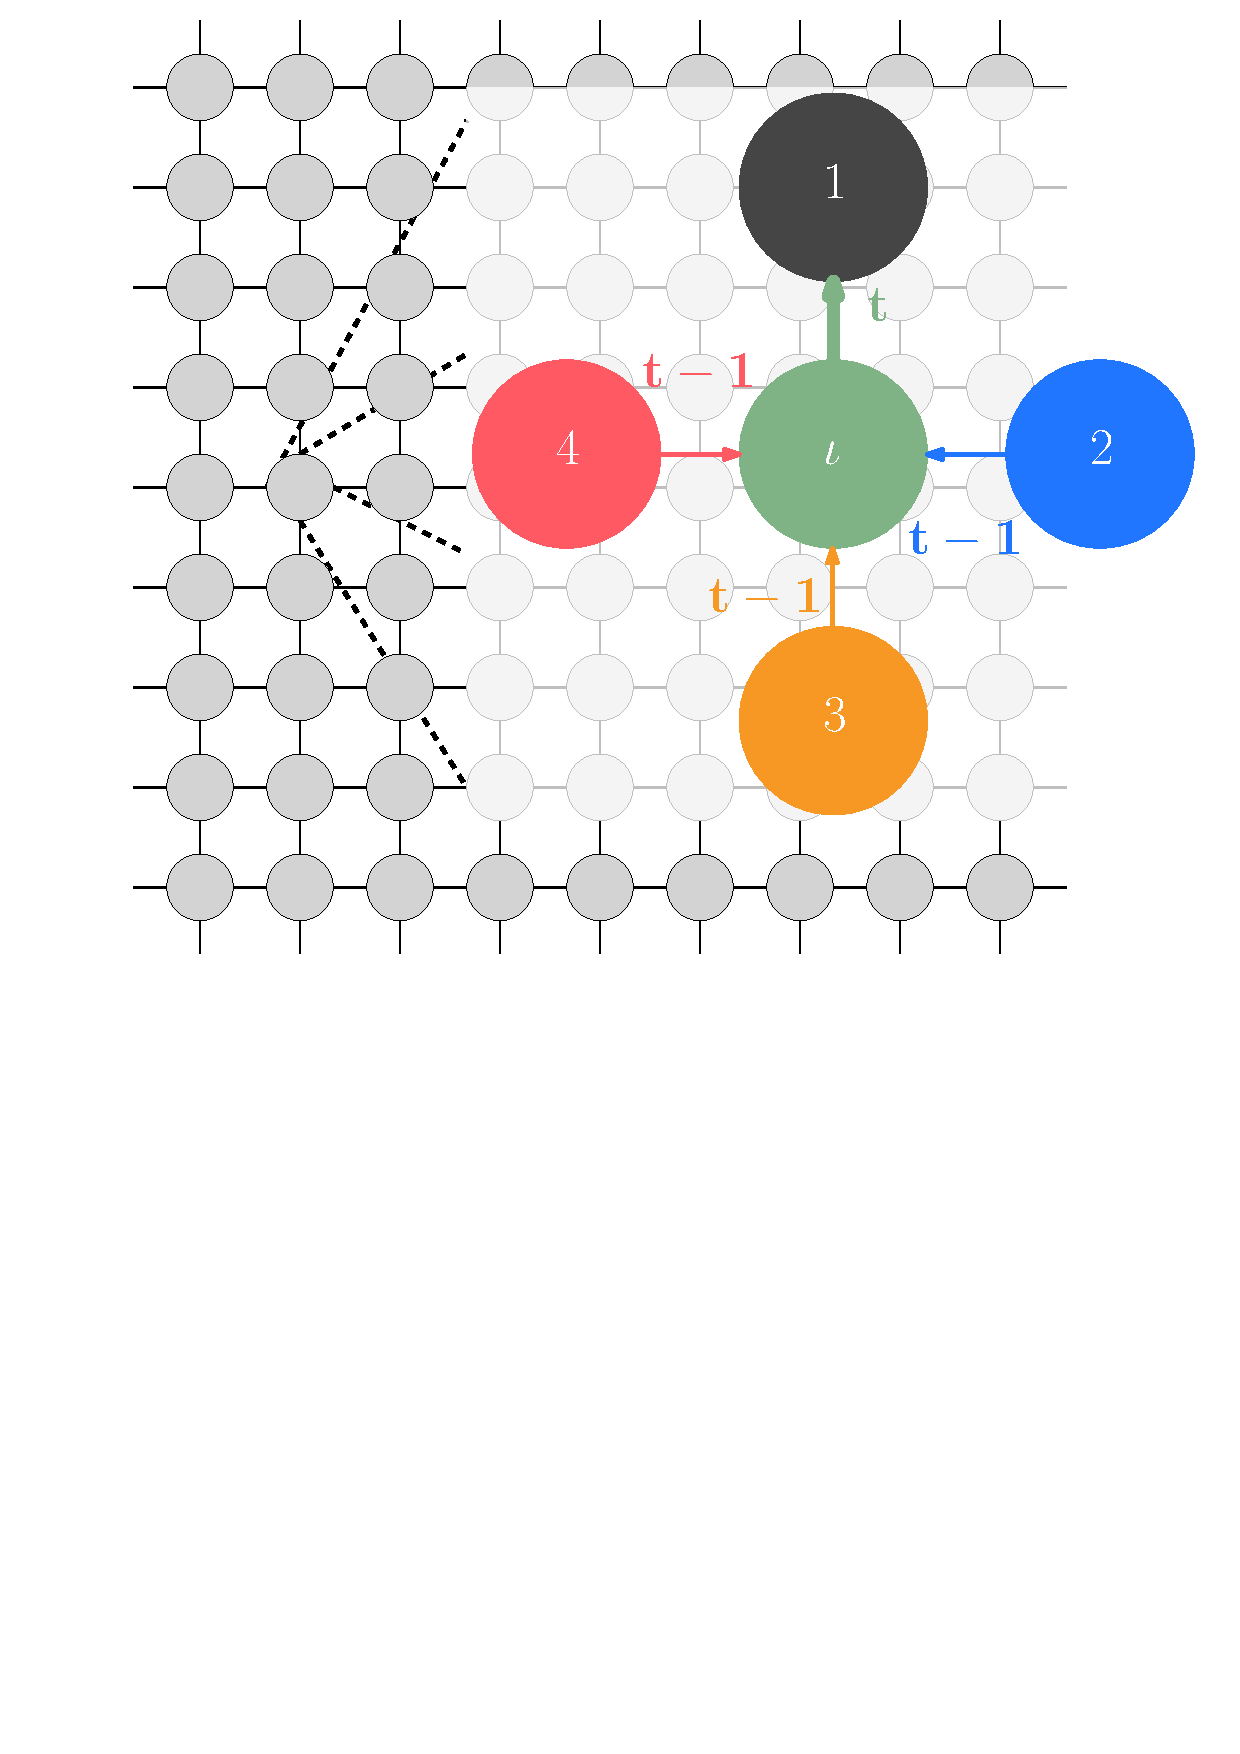
\includegraphics[keepaspectratio,width=1.0\linewidth]{chapters/nmp/images/bp_diagram_recoloured_iotacentre.pdf}
    \caption[Diagram of the central concept of \gls{fne} \glsxtrlong{nmp} on a grid]{Diagram of the central concept of \gls{fne} \gls{nmp} on a grid \cite{lbpmpsmpic}.  Each circle represents a \gls{pe}, labelled following the pattern of \cref{fig:nmp:iota_proxels_environment_oracle}.  The central \gls{pe} \(\iota\) needs to compute a new message to send at time \(t\) to \gls{pe} \(1\) above it, so it performs a computation to combine the results of the messages received from the other three neighbouring cells (\(2\), \(3\) \& \(4\)) at time \(t - 1\) (indicated by the thin and fat arrows).  The same is applied to every other neighbour, too.}
    \label{fig:nmp:gridmessaging}
\end{figure}

Conceptually, there are two distinct aspects of the \gls{nmp} process:
\begin{inparaenum}
\item the message passing itself, which occurs externally to \glspl{pe} over channels connected to other \glspl{pe}; and,
\item the data/message updates, which occur internally.
\end{inparaenum}
The focus of this \namecref{chap:nmp} is the external side, and communication with an oracle stands in for the internal computation, which is largely orthogonal to the inter-\gls{pe} communication.

There are (at least) two separate ways to model the \glspl{pe}' communication:  a \emph{\gls{gs}} system-wide view, where the states and steps taken occur across the system as a whole and every \gls{pe} carries out its operations simultaneously according to the same rules.  Or, a per-\gls{pe} view, where each \gls{pe} has its own state and advances \emph{asynchronously}\footnote{Recall from \vref{sec:back:syncasync} that the idea of asynchronicity used here follows the traditional concept from distributed computing, and so is \emph{different} to that sometimes used in other \gls{ps}.  Briefly, in the asynchronous model of distributed algorithms, external messages may take any arbitrary time (in \(\mathbb{R}\)) to reach their destinations \cite{Balanescu2011,Nicolescu2014,Lynch1996}, though internal updates are typically assumed to occur (near-)instantaneously.} without regard to others' objects, states, and rulesets.  This \namecref{chap:nmp} explores both and finds in the process that an intermediate third, \emph{\gls{ls}}, model arises naturally as a hybrid of the other two.

Modelling and implementation of \gls{nmp} proves surprisingly challenging.  The \gls{gs} form (\cref{sec:nmp:globalsync}) is reasonably simple.  It requires only nine rules, most of which have exactly one term on both the left-hand- and right-hand-sides, and none of which use \glspl{promoter} or \glspl{inhibitor} (see \cref{chap:cpsystems} for more on these concepts).

The challenge arises with the asynchronous version.  The possibility of messages from the same generation arriving at different times necessitates bookkeeping.
% It is necessary to track the sending neighbour from which each message for a given generation is received, to decide which neighbour(s) the current \gls{pe} is now ready to send a new outgoing message.
\Glspl{pe} must track from which neighbours messages have been received for a given generation, to decide to which neighbours the \gls{pe} is ready to send a new message.
This leads to inescapable complexity and the undesirable possibility of deadlock through unsuitable design.

% \Gls{nmp} shares similarities and overlaps with areas such as Cellular Automata, Gossip Protocols and Consensus Algorithms (see \eg{} [INSERT CITATIONS]). \Gls{nmp} is distinguished from these other areas in a few ways, however. Firstly, other approaches do not usually impose the ``\(n - 1\) neighbours'' condition of message updates as found in \gls{nmp}. Secondly, in other areas messaging tends to be only a part of the process, whereas in \gls{nmp} it is the heart of it. Internal computation is only performed to aggregate/average the messages received from neighbours to prepare new messages. Thirdly, in \gls{nmp} neither a global nor local consensus is sought — the closest equivalent would be the (tautological) concept of individual consensus per \gls{pe}. Rather, the result of each \gls{pe} comprises one distinct part of the final result. Lastly, often in these other areas, the neighbours are selected at random, rather than being a neighbourhood arising naturally from the structure of the modelled problem. Generalisation across these fields may be possible, but is not pursued further.
\Gls{nmp} shares similarities and overlaps with areas such as Cellular Automata, Gossip Protocols and Consensus Algorithms (see, \eg{}, \cite{Deserable2012,Hollander2015}).  \Gls{nmp} is distinguished from these other areas in a few ways, however.  Firstly, other approaches do not usually impose the ``\(n - 1\) neighbours'' condition of message updates as found in \gls{nmp}.  Secondly, in other areas messaging tends to be only a part of the process, whereas in \gls{nmp} it is the heart of it.  Internal computation is only performed to aggregate/average the messages received from neighbours to prepare new messages.  Thirdly, neither a global nor local consensus is sought in \gls{nmp} --- the closest equivalent would be the (tautological) concept of individual consensus per \gls{pe}.  Instead, the result of each \gls{pe} comprises one distinct part of the final result.  Lastly, often in these other areas, the neighbours are selected at random rather than being a neighbourhood arising naturally from the structure of the modelled problem.  Generalisation across these fields may be possible but is not pursued further.

This \namecref{chap:nmp} begins by describing a straightforward \gls{gs} \gls{nmp} system.  Then, it provides an asynchronous \gls{pe}-specific version of the same, followed by an adaptation of the asynchronous system to a \gls{ls} system. Next is a short example of a potential evolution of the asynchronous system to clarify its operation.  Lastly, this \namecref{chap:nmp} analyses the asynchronous system and reports the results of comparative computer experiments for all three systems.  The analysis proves that the asynchronous system sends precisely the same number of messages as the \gls{gs} system (one per generation per neighbour) but that the data used to compute new messages may vary slightly depending on the ordering of messages received.  Furthermore, the empirical results verify the operation of the asynchronous system and support the hypothesis that the \gls{ls} and asynchronous systems are faster than an equivalent \gls{gs} version.

\subsection{Belief Propagation}

This \namecref{chap:nmp} was originally motivated by attempts to model \emph{\gls{lbp}} for \gls{sm} (see \eg{} \cite{Blake2011,Felzenszwalb2011,Sun2003}) in \gls{cps}.  \emph{\Gls{bp}} was originally introduced to solve inference problems in AI on graphs \cite{Pearl1982} by treating the nodes as communicating objects, which passed messages backwards and forwards, updating their outgoing messages based on the incoming ones, to solve the problem.  The original formulation relied upon the graphs having a tree structure, however.  Each node would receive a message from its parent, pass that to its children, receive new messages back from the children and pass its own newly computed message back to its parent based on those received from the children.

In the case of \gls{sm}, the output is a (typically rectangular) grid representing an output image.  This means that the computation, sited on this grid, is inherently non-tree-structured.  Instead, each output node is connected to its neighbours -- usually in a \gls{fne} -- which means that messages travel in loops on the grid.  To deal with this situation, \gls{bp} was adapted to \gls{lbp}, which was first applied to \gls{sm} by \citeauthor{Sun2003} \cite{Sun2003}.  The algorithm was then significantly improved upon by \citeauthor{Felzenszwalb2006} \cite{Felzenszwalb2006}.

\Gls{nmp}, as described in this \namecref{chap:nmp}, can simulate \gls{lbp} effectively, and \cref{sec:nmp:example,sec:nmp:analysis,sec:nmp:experiments} focus on the \gls{fne}.  The main adaptation required is to replace the oracle with appropriate computations for \gls{lbp} \gls{sm}.  \Gls{nmp} can be generalised further, however, to perform other computations or use other communication arrangements besides the \gls{fne}.  While this work was originally inspired by \gls{lbp}, it is a generic framework for \emph{any} computations that may be modelled with communication on a lattice, when the outgoing message to one neighbour depends on the messages received from all other neighbours.
% \section{\label{sec:nmp:cpsreview}A Minimal Overview of \texorpdfstring{\gls{cps}}{cP~systems}}
The following is a stripped-down synopsis of \gls{cps}, included in the interests of making this paper more self-contained.  For a comprehensive description and explanation of \gls{cps}, the reader is referred to \cite{Henderson2019,Henderson2020,Nicolescu2018}.

\gls{cps} is another variant of P~systems \cite{Paun2001,Paun2002a,Paun2010b}, complementary to the classic trinity of Cell-like \cite{Paun2000}, Tissue-like \cite{Martin-Vide2003}, and Spiking Neural P~systems \cite{Ionescu2006}.  It has features reminiscent of both Cell-like and Tissue-like systems.  The core unit of \gls{cps} is the \emph{top-level cell}, which is arranged as a nested tree structure, but there can be an arbitrary number of these cells in the environment, communicating with each other through a form of \emph{message-passing over channels}.  The internal operation of \gls{cps}' top-level cells closely resembles Cell-like P~systems.  A key difference, however, is that \emph{only} the top-level cells have accompanying rules.  All sub-cells are merely inert symbolic objects operated upon by the top-level cell's rules.  These sub-cells are represented as labelled multisets within the top-level cells.

Sub-cells can be either \emph{atoms} or \emph{compound terms}, multisets labelled by \emph{functors} (the name `functor' is commonly used as a shorthand for said compound terms).  Atoms, as the name suggests, are indivisible symbols.  They can be of any given type relevant to a system but are static objects with no other inherent properties.  Atoms are written simply as the name of the atom's type.  On the other hand, functors are objects that may hold both atoms and other functors, serve as the said labels for multisets, and are written with the functors' type, followed by opening and closing parentheses surrounding the functor's contents.

Both functors and atoms are written using lower-case letters --- typically from the Latin alphabet, although others may be used.  E.g., an x atom may be written as \(x\), while a y functor might be written like \(\cpfunc{y}{a \, xx \, z}\).  Empty functors are written either with nothing between the parentheses, or with a lower-case lambda: \(\cpfunc{b}{}\) or \(\cpfunc{b}{\cpempty}\).  Furthermore, when there is more than one of a given atom present, the count is usually written as a superscript.  The earlier functor thus could look like \(\cpfunc{y}{a \, x^2 \, z}\).

\emph{Rules} are arguably the most significant difference between \gls{cps} and other P~systems variants.  While \gls{cps} rules still work in a \emph{maximally parallel} \emph{top-down weak-priority order}, update the multisets inside the cells, and depend on the presence of given objects in the cell to make the rules applicable, they also include \emph{variables}.  These variables, written with upper-case letters, are matched with the actual contents of the cells through a one-way unification process \cite{Liu2021}, where the variables are conceptually substituted for contents within a given cell at `run-time'.

Rules are written with exactly one each of a starting \emph{state};\footnote{The states themselves are technically atoms but are not normally used for anything other than specifying the requisite starting and ending states for the top-level cell.} left-hand-side (LHS); \emph{application mode}; ending state; right-hand-side (RHS); followed by zero or more \emph{promoters} and \emph{inhibitors}.  These rules take the form
\begin{framed}
\vspace{-1.0cm}
\cpruleinline{\cprulenonum{s_i}{LHS}{+/1}{s_j}{RHS}}
\vspace{-0.7cm}
\end{framed} 
\noindent
where \(s_i\) is the starting state; \(LHS\) is the multiset of objects required to be present in the given top-level cell and which will be deleted by the rule; \(+/1\) is the application mode, one of either `maximally parallel' or `exactly once', respectively; \(s_j\) is the ending state; \(RHS\) is the multiset of objects that the rule will create.  Maximally parallel application means that the rule is applied as many times at the current step as there are available objects to allow it.  Exactly once mode means that the rule is applied at most one time during a given step.

For example, if a top-level cell has two functors \(a(b^2)\) \& \(\cpfunc{a}{b^3}\), and an applicable rule's LHS is \(a(B)\), \(B\) in this instance will be unified \emph{non-deterministically} to \(b^2\) or \(b^3\).  Or, if the rule uses \(a(bB)\), \(B\) will be unified to \(b\) or \(bb\).  If the rule instead uses \(a(BC)\), then a \emph{non-deterministic} choice will be made to decide what atoms to assign to \(B\) and \(C\), which could be one of the following pairs:  \(B=0\), \(C=2\); \(B=0\), \(C=3\); \(B=1\), \(C=1\); \(B=1\), \(C=2\); \(B=2\), \(C=0\); \(B=2\), \(C=1\); \(B=3\), \(C=0\).

Promoters are objects that \emph{must} be present within the cell for an associated rule to be applicable but are \emph{not} destroyed by the rule.  Conversely, inhibitors are objects that \emph{must not} be present for the rule to be applicable, although the rule may create them.  If promoters are present, they are denoted following a \(|\) per promoter, and inhibitors by \(\neg\), e.g., \(|\,a(A)\) or \(\neg\,b(B)\).  Inhibitors and promoters traditionally are written below the main rule body, but this is not strictly needed.

\begin{framed}
\vspace{-1.1cm}
\begin{align*}
    \text{Promoter:}&\, | ~ \cpfunc{a}{A} & \text{Inhibitor:}&\, \neg ~ \cpfunc{b}{B}
\end{align*}
\vspace{-0.8cm}
\end{framed}

Top-level cells may exchange messages over channels.  Each top-level cell may hold one or more appropriately labelled endpoints for any relevant channels, and may in its rules try both to send and receive messages via those endpoints.  A message is written inside braces and marked either on the RHS with an exclamation mark or on the LHS with a question mark to represent sending or receiving.  E.g., \(\cpsend{\cpfunc{a}{b}}{c}\) would represent a message \(\cpfunc{a}{b}\) to be sent via channel \(c\), and \(\cprecv{\cpfunc{d}{e}}{f}\) would represent a message to be received via channel \(f\).

\begin{framed}
\vspace{-1.1cm}
\begin{align*}
    \text{Send:}&\, \cpsend{\cpfunc{a}{b}}{c} & \text{Receive:}&\, \cprecv{\cpfunc{d}{e}}{f}
\end{align*}
\vspace{-0.8cm}
\end{framed}

Both sending and receiving use pattern matching.  For sending, any \gls{cps} term matching the pattern in the rule may be removed from the top-level cell and passed to a waiting recipient or placed into a buffer multiset in the channel.  Receiving works similarly in that any object matching the pattern of a receipt rule either offered by a top-level cell on the other side of the endpoint or stored in the channel's buffer multiset may be withdrawn.  If more than one object in the buffer matches the pattern, one is selected randomly.  Importantly, this means that ordinary \gls{cps} channels do \emph{not} behave as FIFO queues.

Numerical operations are simulated with unary arithmetic (see, e.g., \cite{Aman2019,Bonchis2006}).  Natural numbers are represented by counting copies of the \emph{unary digit} atom, \(\cpundig\), inside a given functor.  E.g., the number three can be represented as \(\cpfunc{a}{\cpundig\cpundig\cpundig}\), \(\cpfunc{a}{\cpundig^3}\) or \(\cpfunc{a}{3}\).

\begin{framed}
\vspace{-1.1cm}
    \begin{align*}
        \text{Empty functor:}&\, \cpfunc{e}{\cpempty} & \text{The number three:}&\, \cpfunc{a}{\cpundig\cpundig\cpundig} \text{ or } \cpfunc{a}{\cpundig^3} \text{ or } \cpfunc{a}{3}
    \end{align*}
\vspace{-0.8cm}
\end{framed}

Like most other P~systems families, \gls{cps} typically evolve synchronously in a stepwise fashion following an implicit global clock.  Rules are applied based on whether the available multiset(s) within the system match the rules' LHS \& promoters and not the inhibitors.  The consumption of removed objects plus the creation of new objects happens instantaneously at the end of a step.

\subsection{\label{sec:nmp:notation}\texorpdfstring{\gls{cps}}{cP systems} Notation}
A specific cP~system can be described as a 6-tuple, as shown below.

\begin{framed}
\vspace{-1.0cm}
\[
\Pi_{cP}(T, A, O, R, S, \bar{s})
\]
\vspace{-0.7cm}
\end{framed}

\(T\) is the set of top-level cells at the start of the evolution of the system; \(A\) is the alphabet of the system; \(O\) is the set of multisets of initial objects in the top-level cells; \(R\) is the set of rulesets for each top-level cell; \(S\) is the set of possible states of the system; \(\bar{s} \in S\) is the starting state of the system.

\subsection{\label{sec:nmp:compoundterms}Indexed notation for compound terms}

Indexed compound terms appear commonly in \gls{cps} definitions.  These are terms that are tagged in some manner by one or more sub-terms used to distinguish different instances of the same functor type.  They are still classic \gls{cps} objects with nested terms, but some of the said sub-terms are used only to distinguish between instances of the encapsulating compound term.  This is roughly analogous to tagging a term with its index in a logical vector/array, or the key it would be stored under in a typical dictionary/associative array data structure.

For example, later in this paper, compound \(v\) terms appear in multiple rules.  Ordinarily, these would be represented as nested terms like 
\begin{framed}
\vspace{-1.0cm}
\[ \cpfunc{v}{\cpfunc{v'}{X} \; \cpfunc{v''}{G}\; D} \]
\vspace{-0.7cm}
\end{framed}\noindent
and used inside a given \gls{pe} to represent a set of tagged data.  They are indexed by neighbour \(X\) and tagged with a `generation count' \(G\) (further explained in \cref{sec:nmp:pespecific}).  Both values track metadata about a datum.  Lastly, the final datum \(D\) stored by the encapsulating term is given.  In many common programming languages, accessing each datum might be written like \texttt{v[X]}, where \texttt{v} is a dictionary indexed by neighbour.

The \(v\) functors could instead be written as
\begin{framed}
\vspace{-1.0cm}
\[ \cpvv{X}{G}{D} \]
\vspace{-0.7cm}
\end{framed}\noindent
for a shorthand that can be expanded back out to a full form automatically.  The first pair of parentheses selects functors by neighbour, the second records the generation, while the final pair shows the actual contents.  This shorthand is \emph{purely} a notational convenience without effect on rule application and system evolution.  When a concrete instance of a \(v\) compound term is indexed by a ground term (i.e., not a variable) \(k\), e.g. \(\cpvv{k}{\_}{\_}\), we refer to it as \emph{k-tagged}.

\begin{framed}
\vspace{-1.1cm}
    \begin{align*}
        \text{Nested functor:}&\, \cpfunc{v}{\cpfunc{v'}{X} \; \cpfunc{v''}{G}\; D} & \text{Compound term:}&\, \cpvv{X}{G}{D}
    \end{align*}
\vspace{-0.8cm}
\end{framed}

\subsection{\label{sec:nmp:blocking}Blocking vs non-blocking message receipt in \texorpdfstring{\gls{cps}}{cP systems}}
In \gls{cps} sending messages from one top-level cell to others is non-blocking by default because the channels connecting the cells buffer message objects if needed. Thus an outgoing message is always accepted by the mediating channel, even if the holder of the other channel endpoint is not ready to receive the message.  Receiving messages via channels is also ordinarily a non-blocking operation in \gls{cps}, albeit for a different reason.  If there are no eligible messages on the channel, either buffered by the channel itself or offered by the cell holding the other end of the channel, then the relevant rule to receive over that channel will not apply, regardless of whatever other rules may or may not be applied.

It may be useful in some circumstances, however, to simulate the nature of a blocking receipt.  This can be achieved with the use of added dedicated states.  The beginning state for the intended blocking receipt should be unused as the beginning state for any other rule (except for another aspect of the same blocking receipt).  This state is the ending state for another rule, which enters the blocking receipt.  The ending state for the blocking receipt rule should return the cell to its standard process.

The overall effect of using the dedicated state ensures that no other rules may be used inside a particular top-level cell at a given step.  Effectively, the top-level cell becomes quiescent until another top-level cell offers to send a message to the first cell.  At that point, one or more messages are exchanged as appropriate, and the receiving top-level cell returns to its standard processing otherwise.  We make use of this later in \cref{sec:nmp:pespecific} (rules 7 \& 10 in \cref{ruleset:nmp:proxspec}).

As an example, consider the two \gls{cps} rules below:
\begin{framed}
\vspace{-0.3cm}
\cpruleinline{\cprulenonum{s_2}{\cprecv{\cpfunc{x}{Y}}{z}}{+}{s_3}{\cpfunc{x}{Y}}}
\cpruleinline{\cprulenonum{s_2}{}{1}{s_4}{}}
\vspace{-0.7cm}
\end{framed}\noindent
Assume these two rules are the only ones in the ruleset that begin in state \(s_2\) and that the top-level cell this ruleset applies to is presently in state \(s_2\).  Therefore, the only rules which may be applied at the next step are one or the other of these --- the different ending states prevent the application of both.

When applied in the typical top-down weak priority order, the first rule has priority.  If one or more messages available on channel \(z\) match the pattern -- here a functor \(x\) with any contents -- then the first rule applies, and the new \(x\) terms are created in the top-level cell at the end of the step.  Conversely, if no such message is on hand, the top-level cell will unconditionally transition to state \(s_4\).  Thus, receiving messages through the first rule while the second is available is a \emph{non-blocking} receipt.

What if, however, the second rule was not there? If the only rule with the starting state \(s_2\) was the first of those rules?  In that case, the top-level cell will be unable to make progress until at least one matching message becomes available via channel \(z\).  Thus, receiving messages through the first rule \emph{without} the second rule being available is a \emph{blocking} receipt.  The top-level cell is blocked from evolving further and making any forward progress until a suitable message arrives.  It is quite possible for blocking receipt rules to lead to potential deadlocks in a communicating system, and care must be taken to avoid the possibility, akin to any other concurrency scenario.

\subsection{\label{sec:nmp:antiport}Antiport communication rules in \texorpdfstring{\gls{cps}}{cP systems}}

We propose and use an antiport rule \cite{Orellana-Martin2019,Paun2002} in \cref{sec:nmp:systemwide}.  To the best of our knowledge, this is the first time an antiport rule has been used in \gls{cps}.  In brief, antiport rules allow for the bidirectional exchange of objects between membranes/cells/neurons during a single rule execution, with the restriction that objects \emph{must} travel in both directions.  Thus, if one side is only ready to send or receive, rather than both, the rule cannot run at the next step.  Instead, other rules down the priority order will be tested.  An important ramification of this is that it avoids deadlock by both sides of the exchange waiting on the other to send a message.

In the context of \gls{cps}, this means that a given rule must involve a receipt over a channel on the LHS, and a send on the \emph{same} channel on the RHS.  For example,
\begin{framed}
\vspace{-1.0cm}
\cpruleinline{ \cprulenonum{s_1}{\cpantirecv{\cpfunc{a}{B}}{c} \; \cpfunc{d}{E}}{1}{s_2}{\cpantisend{\cpfunc{d}{E}}{c} \; \cpfunc{a}{B}}}
\vspace{-0.7cm}
\end{framed}\noindent
would be valid because the same channel is used on both sides of the rule.  To distinguish clearly between antiport rules and other messaging rules, we write two marks between the message and the channel label, instead of one.
\section{\label{sec:nmp:systemwide}System-wide-synchronicity Messaging}

\cpresetrulenumber

This \namecref{sec:nmp:systemwide} presents the first \gls{nmp} variant, wherein the entire system evolves as one, and every \gls{pe} executes the same rule(s) simultaneously.  For the entirety of this \namecref{chap:nmp}, assume that all \glspl{pe}, channels and the oracle (\(o\)) behave correctly and follow their respective protocols, without faults, corruptions, lost messages, \etc{}  This significantly simplifies the presented systems by allowing the omission of error handling concepts and describing only the intended operation.

\begin{figure}
    \centering
    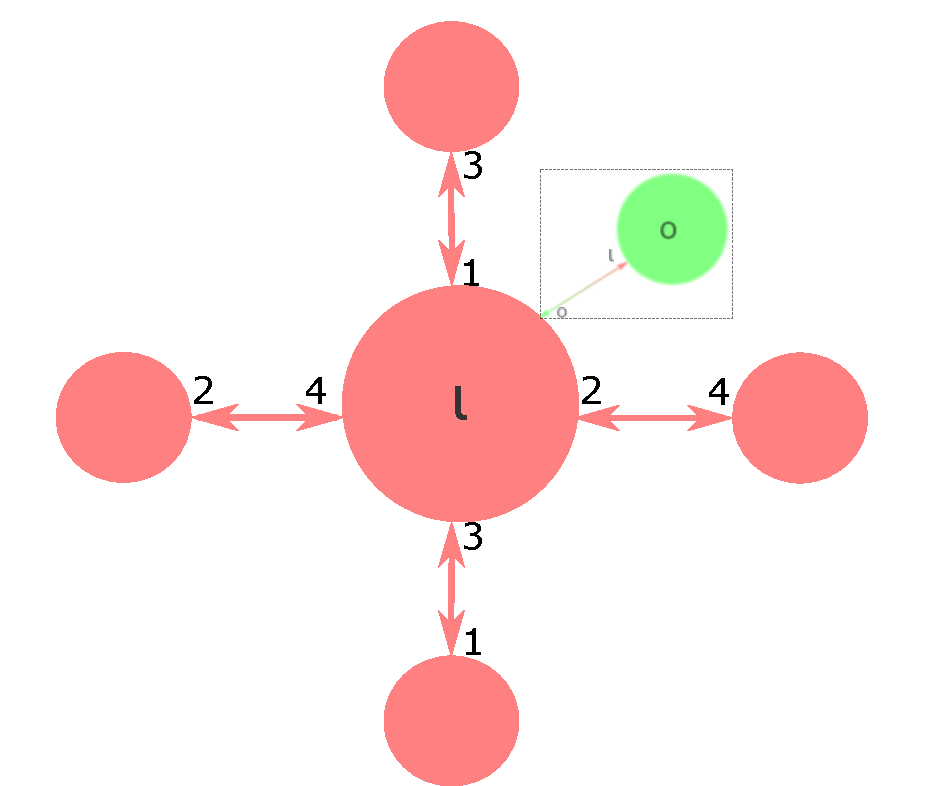
\includegraphics[width=0.9\textwidth]{chapters/nmp/images/iota_proxels_oracle_v7.pdf}
    \caption[The communication topology of a \glsxtrlong{nmp} system from the perspective of an arbitrary \glsxtrshort{pe} in a \gls{fne} arrangement]{The communication topology of the system from the perspective of an arbitrary \gls{pe} in a \gls{fne} arrangement.}
    \label{fig:nmp:iota_proxels_environment_oracle}
\end{figure}

The layout of the system, from the perspective of an arbitrary \gls{pe} in a \gls{fne}, is depicted in \cref{fig:nmp:iota_proxels_environment_oracle}.  The central circle is this \gls{pe} and is labelled with \(\iota\) to represent its ID in the overall system.  It is connected to each neighbour and the oracle by two-way channels.  The neighbours themselves are anonymous, but \(\iota\)'s end of each channel is labelled with a number from 1-4, representing the neighbours who are expected to sit above, to the right, below and to the left of the central \gls{pe}, respectively.  The oracle is smaller, blurred and surrounded with a dashed line, to reflect that it is a stand-in for an unspecified process that ordinarily would take place \emph{inside} the \gls{pe}.

In the current approach, each \gls{pe} has \emph{no} direct knowledge of its neighbouring \glspl{pe}.  Instead, it interacts with channels that connect to those neighbours; the channels interpose between the \glspl{pe}.  Furthermore, each label for a neighbour in a \gls{pe} is \emph{not} the system's ID for that neighbour, but the \gls{pe}'s label for a connecting channel endpoint.  Nevertheless, as a shortcut, \glspl{pe} will simply be referred to as communicating with their neighbours.  Messages exchanged by \glspl{pe} are termed \emph{\gls{nm} messages}, while messages exchanged with an oracle may be referred to as \emph{\gls{oq} messages}.

In the \gls{gs} version, the entire system evolves in lock-step, and thus is always in the same phase and \gls{cps} state.  The evolution follows a basic process, consisting of three conceptually distinct phases, the first two of which may be repeated.  Specifically, the system proceeds as follows (the rules are listed in \vref{ruleset:nmp:systemwide} and explained in \vref{sec:nmp:systemwide:rulesdesc}):

\begin{enumerate}
    % \item\label{enumitem:nmp:init} Initialisation (Rules \cpruleref*{rule:nmp:systemwide:recvcounter} \& \cpruleref*{rule:nmp:systemwide:recvinput})
    \item\label{enumitem:nmp:pu} \Gls{oq} (Rules \cpruleref*{rule:nmp:systemwide:loopdecrement}, \cpruleref*{rule:nmp:systemwide:sendtooracle} \& \cpruleref*{rule:nmp:systemwide:recvfromoracle})
    \item\label{enumitem:nmp:nm} \Gls{nm} (rule \cpruleref*{rule:nmp:systemwide:antiport})
    \item\label{enumitem:nmp:final} \textsf{Finalisation} (Rules \cpruleref*{rule:nmp:systemwide:loopend}, \cpruleref*{rule:nmp:systemwide:oraclefinalise} \& \cpruleref*{rule:nmp:systemwide:end})
\end{enumerate}

% This progression is depicted as a state machine in \cref{fig:nmp:systemwidestatemachine}.  State \(s_1\) covers the initialisation phase; \(s_2\) and \(s_3\) the \gls{oq} phase; \(s_4\) the \gls{nm} phase; and \(s_5\) and \(s_6\) the finalisation phase.  State \(s_7\) is the halting phase of the system's evolution.  In an application of \gls{nmp} phases \ref{enumitem:nmp:init}, \ref{enumitem:nmp:nm} and \ref{enumitem:nmp:final} will not change.  Only phase \ref{enumitem:nmp:pu} would be replaced.  The system's evolution is sketched at a high level in \cref{alg:nmp:systemwide2}.

\Cref{fig:nmp:systemwidestatemachine} depicts this progression as a state machine.  States \(s_1\) and \(s_2\) cover the \gls{oq} phase; \(s_3\) the \gls{nm} phase; and \(s_4\) and \(s_5\) the \textsf{finalisation} phase.  State \(s_6\) is the halting state of the system's evolution.  In an application of \gls{nmp} phases \ref{enumitem:nmp:nm} and \ref{enumitem:nmp:final} will not change.  Only phase \ref{enumitem:nmp:pu} is replaced.  The system's evolution is sketched at a high level in \cref{alg:nmp:systemwide2}.

The \gls{oq} phase is when each \gls{pe} performs its internal computation. As mentioned earlier, these computations are problem-dependent and thus cannot be modelled generically. Instead, this \namecref{chap:nmp} uses communication with an oracle assigned to each \gls{pe} to simulate this aspect of \gls{nmp}. The \gls{nm} phase is the main focus of this work. This is where \glspl{pe} exchange messages with their neighbours, based on data received earlier from other neighbours. The \textsf{finalisation} phase occurs after each \gls{pe} reaches a stopping point. At this point, each \gls{pe} performs a final computation to determine its output for the lattice, incorporating the latest data received from neighbours.

\begin{figure}
    \centering
    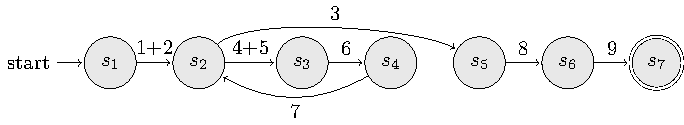
\includegraphics{chapters/nmp/images/systemwidestatemachine.pdf}
    \caption[State machine of the progression of the system-wide \glsxtrlong{nmp} \gls{cps} rules.]{State machine of the progression of the system-wide \gls{nmp} \gls{cps} rules.  The vertices are labelled with states and the arcs with the rule(s) which cause the state transitions.}
    \label{fig:nmp:systemwidestatemachine}
\end{figure}

\begin{algorithm}
\DontPrintSemicolon
\KwIn{Iteration counter \(i\) and array \(v\) of initial data}
\KwOut{Final result \(z\)}
\SetKwFor{pForEach}{parallel foreach}{do}{endfch}
\Begin{
    \tcc{\(\alpha \Leftarrow \langle \beta \rangle\) denotes receiving object \(\alpha\) on channel \(\beta\);\newline\(\gamma \Rightarrow \langle \delta \rangle\) denotes sending object \(\gamma\) on channel \(\delta\);\newline\(\epsilon \Leftrightarrow \langle \phi \rangle\) denotes antiport exchange, sending \emph{and} receiving (swapping) objects \(\epsilon\) on channel \(\phi\).}\;
    
    % \tcc{Initialisation}
    % \(i \Leftarrow \langle e \rangle\)\;
    % \lpForEach{\((x,d) \Leftarrow \langle e \rangle\)}{\(v[x] \gets d\)}\;
    
    \While{\(i > 0\)}{
        \tcc{\Glsentrylong{oq}}
        \(i \gets i - 1\)\;
        \pForEach{\(x \in \{1, 2, 3, 4\}\)}{
            \(w[x] \gets v[x]\)\;
            \(w[x] \Rightarrow \langle o \rangle\)
        }
        \lpForEach{\((x,d) \Leftarrow \langle o \rangle\)}{
            \(v[x] \gets d\)\
        }
        
        \;\tcc{\Glsentrylong{nm}}
        \lpForEach{\(x \in \{1, 2, 3, 4\}\)}{\(v[x] \Leftrightarrow \langle x \rangle\)}
    }
    \;\tcc{\textsf{Finalisation}}
    \pForEach{\(x \in \{1, 2, 3, 4\}\)}{
        \(w'[x] \gets v[x]\)\;
        \(w'[x] \Rightarrow \langle o \rangle\)
    }
    \(z \Leftarrow \langle o \rangle\)\;
    % \(z \Rightarrow \langle e \rangle\)
}
\caption[Pseudocode of the \glsxtrlong{nmp} process in the \gls{gs} system]{\label{alg:nmp:systemwide2}Pseudocode description of the process for an individual \gls{pe} in the \gls{gs} system}
\end{algorithm}

Assume before the start of the system's evolution that the correct number of \glspl{pe} are already in place, and they each contain an appropriately initialised iteration counter and their relevant channel endpoints only.  Everything else required by each \gls{pe} will be supplied by the oracle, or generated by rules during the \gls{pe}'s evolution.  The rules for the \gls{gs} system are listed in \cref{ruleset:nmp:systemwide} and explained in \cref{sec:nmp:systemwide:rulesdesc}.  This \namecref{sec:nmp:systemwide} first defines the \gls{gs} \gls{nmp} system, explains the intended operation of the \gls{ruleset}, then describes each of the ground terms used.

\subsection{System Definition}
Recall from \cref{sec:cps:formaldescriptions} that a given \gls{cps} implementation can be defined as a 6-tuple:

\cptuple{\text{NMP-GS}}{\cpset{\sigma_1, \dots, \sigma_{\text{max}}}}{A}{O}{\text{\cref{ruleset:nmp:systemwide}}}{\cpset{s_1, s_2, s_3, s_4, s_5, s_6}}{s_1}

\(T\) is a set of \glspl{tlc}, each representing a single \gls{pe}, numbered from one to the total size of the lattice.  These numbers correspond to the \(\iota\) of \cref{fig:nmp:iota_proxels_environment_oracle}.  \(A\) is the set of all terms defined in \cref{sec:nmp:systemwide:definitions}.  Each \gls{pe}'s starting multiset in \(O\) is a generation counter functor \(i\) and its set of initial data \(V\).

\subsection{\label{sec:nmp:systemwide:rulesdesc}Description of Rules}

\begin{cprulesetfloat}
    \begin{cpruleset}
        % % Receive maximum generation counter
        % \cprule[rule:nmp:systemwide:recvcounter]{s_1}{\cprecv{\cpfunc{i}{I}}{e}}{\cponce}{s_2}{\cpfunc{i}{I}}
        
        % % Receive inputs from environment
        % \cprule[rule:nmp:systemwide:recvinput]{s_1}{\cprecv{\cpvq{X}{D}}{e}}{\cpmaxpar}{s_2}{\cpvq{X}{D}}
        
        \\
        
        % Else move to finishing
        \cprule[rule:nmp:systemwide:loopend]{s_1}{i(\lambda)}{\cponce}{s_4}{}
        
        % Decrement iterator
        \cprule[rule:nmp:systemwide:loopdecrement]{s_1}{i(I\cpundig)}{\cponce}{s_2}{i(I)}
        
        % Send to oracle
        \cprule[rule:nmp:systemwide:sendtooracle]{s_1}{\cpvq{X}{D}}{\cpmaxpar}{s_2}{\cpsend{\cpvqw{X}{D}}{o}}
        
        % Receive from oracle
        \cprule[rule:nmp:systemwide:recvfromoracle]{s_2}{\cprecv{\cpvqw{X}{D}}{o}}{\cpmaxpar}{s_3}{\cpvq{X}{D}}
        
        \\
        
        % Exchange messages
        \cprule[rule:nmp:systemwide:antiport]{s_3}{\cpvq{X}{D} & & &\\ & \cpantirecv{\cpvq{\_}{D'}}{X}}{\cpmaxpar}{s_1}{\cpvq{X}{D'} &\\ & & & & \cpantisend{\cpvq{X}{D}}{X}}
        
        \\
        
        % Send to oracle (finalisation)
        \cprule[rule:nmp:systemwide:oraclefinalise]{s_4}{\cpvq{X}{D}}{\cpmaxpar}{s_5}{\cpsend{w'\perfectunary{IncreaseHeight}{(}{)}{X}\perfectunary{IncreaseHeight}{(}{)}{D}}{o}}
        
        % Oracle returns results
        \cprule[rule:nmp:systemwide:end]{s_5}{\cprecv{\cpfunc{z}{Z}}{o}}{\cpundig}{s_6}{\cpfunc{z}{Z}}
        
    \end{cpruleset}
    \caption[Complete \gls{ruleset} for \gls{gs} \glsxtrlong{nmp}]{\label{ruleset:nmp:systemwide}Complete \gls{ruleset} for \gls{gs} \gls{nmp}, using an oracle to perform update computations}
\end{cprulesetfloat}

\begin{enumerate}
    % \item Receive \(I\), the maximum generation count or the number of rounds of message passing each \gls{pe} should engage in.\footnote{In general with \gls{nmp} a fixed number of generations is not the only way to determine when \gls{nm} should cease, but other methods tend to be specific to the problem at hand.   Therefore, a generation count is the only one presented here.  It should be applicable no matter the computation performed.}
    % \item Receive from the environment \gls{nm} messages \(v(X)(D)\), being the \gls{pe}'s initial data for its neighbours.
    \item If \(i\) is empty, continue to the \textsf{finalisation} phase.
    \item Decrement \(i\) when sending \(w\) messages to the oracle for \gls{oq}.
    \item Convert the \(v\) messages into \(w\) messages and send them to the oracle to compute the new messages to send to neighbours.
    \item Receive back new \(w\) objects from the oracle and convert them to \(v\) objects.
    \item Swap \(v\) messages with each neighbour \(X\), using antiport communication (see \cref{sec:cps:antiport}).
    \item Send the \(v\) objects as \(w'\) to the oracle for \textsf{finalisation} computation.
    \item Receive the final result \(\cpfunc{z}{Z}\) from the oracle and halt.% and send it to the environment.\footnote{One might wonder why the oracle could not simply emit the final result directly into the environment.  Strictly speaking, that would be reasonable in the context of this system, but bear in mind that the oracle is simply an abstraction over an arbitrary computation, which would take place \emph{inside} the \gls{pe}.}
\end{enumerate}

\subsection{\label{sec:nmp:systemwide:definitions}Definitions of Terms}

\paragraph{Atoms}
\begin{description}
    % \cptermdef{e}{The label of the channel used to communicate with the environment.}
    \cptermdef{o}{The label of the channel used to communicate with the oracle.}
    \cptermdef{\cpempty}{The \gls{cps} `empty' atom (see \cref{sec:cps:complexsymbols,sec:cps:natnums}).}
\end{description}

\paragraph{Functors}
\begin{description}
    \cptermdef{i}{A generation counter.  Used to count the number of generations of \gls{nm} remaining before moving to the \textsf{finalisation} phase.}
    \cptermdef{v}{The \(v\) compound terms described in \cref{sec:cps:compoundterms} \emph{except} without the generation counter --- the \(i\) counter serves the same purpose for the \gls{gs} variant.  These serve as \gls{nm} messages.}
    \cptermdef{w}{The same as the \(v\) terms, but used as messages to the oracle for \gls{oq}.}
    \cptermdef{w'}{The same as the above \(w\) objects, but marked to indicate to the oracle that they are to be used for \textsf{finalisation} rather than \gls{oq}.}
    \cptermdef{z}{Final output functor.  Holds the result of the \gls{pe}’s computation.}
\end{description}

\paragraph{States}
\begin{description}
    % \cptermdef{s_1}{Beginning state.  The \glspl{pe} receive their inputs from the environment.}
    \cptermdef{s_1}{The opening \gls{oq} phase state, where data are sent to the oracle and the generation counter is decremented.}
    \cptermdef{s_2}{Data update receipt state. Updated data are received back from the oracle.}
    \cptermdef{s_3}{\Gls{nm} state.  Messages are swapped with neighbours.}
    \cptermdef{s_4}{\textsf{Finalisation} phase transition state}
    \cptermdef{s_5}{State for transmission to the oracle for the final result, and awaiting its response.}
    \cptermdef{s_6}{State for receipt of the result from the oracle and halting of evolution.}
\end{description}
\section{\label{sec:nmp:pespecific}Processing Element-specific Asynchronous Messaging}
% \cpresetrulenumber

This \lcnamecref{sec:nmp:pespecific} presents a variant of the above system where the rules are applied in a \gls{pe}-specific manner and the \glspl{pe} run \emph{asynchronously} \cite{Balanescu2011,Nicolescu2014}, so that the steps of one \gls{pe} do not necessarily occur contemporaneously with those of another.\footnote{In this form, \gls{nmp} shares some obvious similarities with \Gls{csp} (\cref{subsec:back:csp}), \Glspl{actor} (\cref{subsec:back:actors}) and \Glspl{pram} (\cref{sec:back:othermodels}).}  

\begin{anfxwarning}{Keep and modify this paragraph, or delete it?}
There is no longer a single state spanning the entire system.  Instead, each \gls{pe} has its own state dictating its operation individually.  The same conceptual phases are kept, though the \gls{oq} and \gls{nm} phases are combined because they now may occur interleaved.  During the \gls{oq} \& \gls{nm} phase, each \gls{pe} independently works through a series of \label{pg:nmp:rounds}\emph{rounds}, following the typical idea of a round in theoretical asynchronous systems:  The \gls{pe} receives one or more messages, processes the received messages and updates its internal data, then sends out new messages based on the results.
\end{anfxwarning}

The most significant change from \cref{sec:nmp:systemwide} is the use of \emph{receipt tokens} and \emph{generation counts}.  Receipt tokens show that the \gls{pe} has received a message from a particular neighbour since the last time messages were sent.  This is vital to ensure that the correct number of messages are sent, and sent only after receiving appropriate messages from other neighbours.

In the \gls{gs} system, the received messages used to update the outgoing messages could always be assumed to have been sent during the same round as each other.  This is not the case under the asynchronous system, where a message may be sent out (and thus received) as soon as the necessary input messages have been received.  This has the potential to messages being used out-of-order, where a message from what would have been an earlier `round' is re-used inappropriately.  Thus, these messages are now tagged with a round number, termed here a \emph{generation} because each outgoing message is essentially the direct progeny of the messages received at the last generation.

The other change of note is that initialisation of the \glspl{pe} also differs slightly from \cref{sec:nmp:systemwide}.  Along with the channels, each \gls{pe} also starts with an adjacency list object, \(\cpfunc{a}{A}\), which holds a copy of the atoms for each neighbour/channel.

\begin{figure}
    \centering
    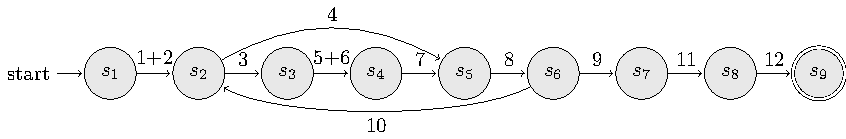
\includegraphics[width=1.0\textwidth]{chapters/nmp/images/proxelspecificstatemachine.pdf}
    \caption[State machine of the progression of the \glsxtrshort{pe}-specific \glsxtrlong{nmp} \gls{cps} rules]{State machine of the progression of the \gls{pe}-specific \gls{nmp} \gls{cps} rules.  The vertices are labelled with the states and the arcs with the rule(s) which cause that transition.}
    \label{fig:nmp:proxelspecificstatemachine}
\end{figure}

As with \cref{sec:nmp:systemwide}, this \lcnamecref{sec:nmp:pespecific} shows the progression of the system through its states in \cref{fig:nmp:proxelspecificstatemachine}.  In this system, an \gls{oq} \& \gls{nm} round can be regarded as the steps taken to proceed from state \(s_2\) until reaching \(s_2\) again.  Thus, receiving one or more messages, followed potentially by preparing and sending new messages, forms a round.  The initialisation phase is only rules \cpruleref*{rule:nmp:proxspec:initcounter} and \cpruleref*{rule:nmp:proxspec:recvinputs}.  The combined \gls{oq} and \gls{nm} phase is made up of rules \cpruleref*{rule:nmp:proxspec:makews} through \cpruleref*{rule:nmp:proxspec:recvfromneighs}, which involve the receipt of one or more messages with generation \(0 < g \leq I\) from neighbours, then preparation of new messages to send to neighbours through communicating with the oracle and forwarding the results of the oracle's computation to the relevant neighbours.  Lastly, rules \cpruleref*{rule:nmp:proxspec:finaloracle} and \cpruleref*{rule:nmp:proxspec:end} make up the finalisation phase.

\begin{algorithm}
\DontPrintSemicolon
\SetKwFunction{Uniq}{uniq}
\SetKwFunction{Perm}{permutations}
\SetKwFor{pForEach}{parallel foreach}{do}{endfch}
\SetKwBlock{Loop}{loop:}{}
\SetKw{KwOr}{or}
\SetKw{KwAnd}{and}
\SetKw{KwGoto}{goto}
\KwIn{Adjacency set \(A = \{1,2,3,4\}\)}
\KwOut{Final result, \(z\), sent to environment \(e\)}
\Begin{
    \tcc{
    \(a \Leftarrow \langle b \rangle\) denotes receiving object \(a\) on channel \(b\)\newline
    \(c \Rightarrow \langle d \rangle\) denotes sending object \(c\) on channel \(d\)
    }\;
    
    \tcc{Initialisation}
    \(R \gets \emptyset\)\;
    \(i \Leftarrow \langle e \rangle\)\;
    
    \tcc*[l]{* assume environment \(e\) sends all of these now}
    \pForEach{\((x, 0, d) \Leftarrow \langle e \rangle\)}{
        \(v[x] \gets (0,d)\)\;
        \(R \gets R \cup \{x\}\)
    }
    
    \;\tcc{\Glsentrylong{oq} \emph{and} \Glsentrylong{nm}}
    
    \Loop{
        \(W \gets \emptyset\)\;
        
        \pForEach{\((x,y,z,w) \in\) \Perm{\(A\)}}{
            \If{\(x \in R\) \KwAnd \(v[x].g < i\) \KwAnd \(v[x].g \leq v[y].g\) \KwAnd \(v[x].g \leq v[z].g\)}{
                \(W \gets W \cup (w,v[x].g+1, v[x].d \cup v[y].d \cup v[z].d))\)\label{line:nmp:rule3}
            }
        }
        
        \If{\(W \not= \emptyset\)}{
            \(W \gets\) \Uniq{\(W\)} \tcc*[l]{Multiset to set}
            \;
            \lpForEach{\((w, g, d) \in W\)}{\((w, g, d) \Rightarrow \langle o \rangle\)}
            \tcc*[l]{** assume oracle \(o\) returns all required messages}
            
            \lpForEach{\((w, g, d) \Leftarrow \langle o \rangle\)}{\((w, g, d) \Rightarrow \langle w \rangle\)}
            \(W \gets \emptyset\)
        }
        
        \(R \gets \emptyset\)\;
        \;
        \(b \gets\) \texttt{true}
        
        \lpForEach{\(x \in A\)}{\lIf*{\(v[x].g < i\)}{\(b \gets\) \texttt{false}}}
        \lIf{b}{\KwGoto break}\;
        
        \While{\(|R| = 0\)}{\label{line:nmp:recvwhile}
            \pForEach{\((x, g, d) \Leftarrow A\)}{\label{line:nmp:recvfor}
                \(v[x] \gets (g,d)\)\;
                \(R \gets R \cup \{x\}\)\;
            }
        }
        \KwGoto loop\;
    }
    \AlCapSty{\AlCapFnt break:}\;
    
    \;\tcc{Finalisation}
    
    \lpForEach{\(x \in A\)}{\(v[x] \Rightarrow \langle o \rangle\)}
    \(z \Leftarrow \langle o \rangle\)\;
    \(z \Rightarrow \langle e \rangle\)
}
\caption[Pseudocode description of the process for an individual \gls{fne} \glsxtrshort{pe} in the asynchronous system]{\label{alg:nmp:pespecific}Pseudocode description of the process for an individual \gls{fne} \gls{pe} in the asynchronous system}
\end{algorithm}

As with \cref{sec:nmp:systemwide}, this \lcnamecref{sec:nmp:pespecific} also supplies a pseudocode representation of the procedure in \cref{alg:nmp:pespecific}.  The pseudocode does not closely resemble \cref{ruleset:nmp:proxspec} in appearance.  Instead, the pseudocode is written to reflect best the meaning and intention of the rules while still relating it to the \gls{ruleset}.

An important assumption for this \gls{ruleset} is that the oracle returns all outstanding results together.  After a \gls{pe} sends one or more \gls{oq} messages to the oracle, it enters a blocking wait until it receives updated \gls{nm} messages back from the oracle.  One \gls{nm} message is expected per \gls{oq} message.  The oracle is assumed to return all these messages during one step, possibly waiting until it has finished computing new values for every message.  The same assumption is made for finalisation, and similarly, that the environment sends in all the initial messages during a single step.

In preparing the new \gls{oq} messages to go to the oracle, \cpruleref{rule:nmp:proxspec:makews} discards the information about which datum came from which neighbour (visible in \cref{line:nmp:rule3} in \cref{alg:nmp:pespecific}).  This is irrelevant for \gls{bp} \gls{sm}.  It might be relevant, however, to keep said information for a different computation.  One must bear this in mind when adapting the rules to their problem.  The changes needed are likely minor, but unexplored further here, as they are superfluous.

\subsection{System Definition}
Per the tuple definition from \cref{sec:cps:formaldescriptions}:

\cptuple{\text{NMP-Async}}{\cpset{\sigma_1, \dots, \sigma_{\text{max}}}}{A}{\cpset{\cpfunc{a}{A_t} \, | \, t \in T}}{\cref{ruleset:nmp:proxspec}}{\cpset{s_1, \dots, s_9}}{s_1}

\(T\) is a set of top-level cells, each representing a single \gls{pe}, numbered sequentially.  These numbers correspond to the \(\iota\) of \cref{fig:nmp:iota_proxels_environment_oracle}.  \(A\) is equal to the set of terms defined in \cref{sec:pespecific:definitions}.  Each \gls{pe}'s starting multiset in \(O\) is the appropriate channel endpoints and an adjacency list term \(a\), with contents \(A_t\) listing its neighbours specifically.  Every \gls{pe}'s \gls{ruleset} in \(R\) is either equal to that found in \cref{ruleset:nmp:proxspec}, or one which starts with that \gls{ruleset} as a base.  These latter \glspl{ruleset} drop terms from \cpruleref{rule:nmp:proxspec:makews} to adapt it to the relevant \gls{pe} having fewer than four neighbours (see \cref{sec:nmp:ruleslessthanfour}).

\subsection{Description of Rules}

\begin{cprulesetfloat}
    \begin{cpruleset}
    
        %%%%%%%%%%%%%  Initialisation  %%%%%%%%%%%%%
    
        % Receive inputs from environment
        \cprule[rule:nmp:proxspec:initcounter]{s_1}{\cprecv{\cpfunc{i}{I}}{e}}{\cponce}{s_2}{\cpfunc{i}{I}}
        
        \cprule[rule:nmp:proxspec:recvinputs]{s_1}{\cprecv{\cpvv{X}{\cpempty}{D}}{e}}{\cpmaxpar}{s_2}{\cpvv{X}{\cpempty}{D} & \\ & & & & \cpfunc{r}{X}}
        
        \\
        
        %%%%%%%%%%%%%  OQ & MP phase  %%%%%%%%%%%%%
        
        \cprule[rule:nmp:proxspec:makews]{s_2}{}{\cpmaxpar}{s_3}{\cpvw{W}{G\cpundig}{\cpfunc{d}{A}\,\cpfunc{d}{B}\,\cpfunc{d}{C}}}
        \cppromoter{\cpfunc{r}{X}}
        \cppromoter{\cpvv{X}{G}{A}}
        \cppromoter{\cpvv{Y}{G\cpdiscard}{B}}
        \cppromoter{\cpvv{Z}{G\cpdiscard}{C}}
        \cppromoter{\cpfunc{i}{G\cpundig\cpdiscard}}
        \cppromoter{\cpfunc{a}{\cpfunc{n}{X}\,\cpfunc{n}{Y}\,\cpfunc{n}{Z}\,\cpfunc{n}{W}}}
        
        \cprule[rule:nmp:proxspec:skiptorecv]{s_2}{}{\cponce}{s_5}{}
        
        \cprule[rule:nmp:proxspec:uniq]{s_3}{\cpvw{W}{\cpdiscard}{\cpdiscard}}{\cpmaxpar}{s_4}{}
        \cppromoter{\cpvw{W}{\cpdiscard}{\cpdiscard}}
        
        % Send to oracle
        \cprule[rule:nmp:proxspec:sendtooracle]{s_3}{\cpvw{W}{G}{D}}{\cpmaxpar}{s_4}{\cpsend{\cpvw{W}{G}{D}}{o}}
        
        % Receive from oracle & send to neighbour
        \cprule[rule:nmp:proxspec:recvfromoracle]{s_4}{\cprecv{\cpvw{W}{G}{D}}{o}}{\cpmaxpar}{s_5}{\cpsend{\cpvv{W}{G}{D}}{W}}
        
        % Clear all receipt tokens at the end of a send process
        \cprule[rule:nmp:proxspec:clearrs]{s_5}{\cpfunc{r}{\cpdiscard}}{\cpmaxpar}{s_6}{}
        
        % Transition to end if all generations complete
        \cprule[rule:nmp:proxspec:movetoend]{s_6}{}{\cponce}{s_7}{}
        \cpinhibitor{\cpvv{X}{G}{D}}
        \cppromoter{\cpfunc{i}{G\cpundig\cpdiscard}}
        
        %receive messages
        \cprule[rule:nmp:proxspec:recvfromneighs]{s_6}{\cprecv{\cpvv{\cpdiscard}{G\cpundig}{D}}{X} & & & \\ & \cpvv{X}{G}{\cpdiscard}}{\cpmaxpar}{s_2}{\cpvv{X}{G\cpundig}{D} &\\ & & & & \cpfunc{r}{X}}
        
        \\
        
        %%%%%%%%%%%%%  Finalisation %%%%%%%%%%%%%
        
        % Send to oracle
        \cprule[rule:nmp:proxspec:finaloracle]{s_7}{\cpvv{X}{G}{D}}{\cpmaxpar}{s_8}{\cpsend{w'\perfectunary{IncreaseHeight}{(}{)}{X}\perfectunary{IncreaseHeight}{(}{)}{G}\perfectunary{IncreaseHeight}{(}{)}{D}}{o}}
        
        % Oracle returns results which are immediately emitted to the environment
        \cprule[rule:nmp:proxspec:end]{s_8}{\cprecv{\cpfunc{z}{Z}}{o}}{\cpundig}{s_9}{\cpsend{\cpfunc{z}{Z}}{e}}
        
    \end{cpruleset}
    \caption[\Gls{ruleset} for the \glsfmttext{fne} \glsxtrshort{pe}-specific asynchronous \glsfmttext{nmp} system, for an inner \glsxtrshort{pe}]{\label{ruleset:nmp:proxspec}\Gls{ruleset} for the \gls{fne} \gls{pe}-specific asynchronous \gls{nmp} system, for an inner \gls{pe} (\ie{} one not on the border) and using an oracle to compute the data for outgoing messages}
\end{cprulesetfloat}

\begin{enumerate}
    \item Receive the \(\cpfunc{i}{I}\) input from the environment.
    \item Receive \(\cpvv{X}{\cpempty}{D}\) messages as inputs from the environment.
    \item Consider in turn all receipt tokens \(r\), if any (in any arbitrary order). For \(\cpfunc{r}{k_1}\) and \(\cpvv{k_1}{g_1}{\cpdiscard}\), compare generation number \(g_1\) against the generation numbers of all other current values \(\cpvv{k_j}{g_j}{\cpdiscard}, k_j \in \{k_2, k_3, k_4\} = \{1, 2, 3, 4\} \setminus \{k_1\}\). Without loss of generality, if \(g_1 \leq g_2, g_3\) \emph{and} \(g_1 < I\) (\ie{} the maximum generation count) then create a message \(w\) to send to the oracle for \gls{oq}.  This message has the data for \(k_1\), \(k_2\) and \(k_3\), which are used by the oracle in computing the new message to send to \(k_4\).  The generation count for this \(w\) message is \(g_1 + 1\).
    \item If there were no \gls{oq} messages generated by \cpruleref{rule:nmp:proxspec:makews}, then move straight to the process of testing for termination and receiving new messages.
    \item If \cpruleref{rule:nmp:proxspec:makews} resulted in the creation of more than one \gls{oq} message about a given neighbour, select one of those messages at random and delete the others.  The messages will be identical, but duplicates may arise due to the unification of different neighbours to \(Y\) and \(Z\) in \cpruleref{rule:nmp:proxspec:makews}.
    \item For each \gls{oq} message remaining after \cpruleref{rule:nmp:proxspec:uniq}, send said message to the oracle to compute the new corresponding outgoing \gls{nm} message.
    \item Forward newly prepared \gls{nm} messages \(v\) from the oracle to the relevant neighbour.
    \item Delete all extant receipt tokens after completing the relevant \gls{oq} \& \gls{nm} phase.
    \item If messages with a generation count equal to \(I\) have been received from every neighbour, transition to the finalisation phase.
    \item Receive a message \(\cpvv{\cpdiscard}{G}{D}\) from neighbour \(X\) and replace the current \(v\) object for \(X\) with it.  The neighbour label contained inside the message is overwritten with the current \gls{pe}'s label for the receiving channel.  Create a receipt token \(\cpfunc{r}{X}\).
    \item Send all the \gls{pe}'s \(v\) messages to the oracle, for the oracle to compute the final output for the \gls{pe}.
    \item Receive the computed final result from the oracle and send it to the environment.
\end{enumerate}

\subsection{\label{sec:pespecific:definitions}Definitions of Terms}

\paragraph{Atoms}
The same as in \cref{sec:nmp:systemwide}.

\paragraph{Functors}
\begin{description}
    \cptermdef{a}{Adjacency set.  Lists the neighbours of the \gls{pe} as a set of \(n\) functors.}
    \cptermdef{i}{Maximum generations counter.  Used slightly differently to \cref{sec:nmp:systemwide}.}
    \cptermdef{n}{Neighbourhood functor.  Stores the label for one of the channels/neighbours to which the current \gls{pe} is connected.}
    \cptermdef{r}{Receipt token, showing that a message was recently received from neighbour \(X\).}
    \cptermdef{v}{Serves as both the internal data stores and \gls{nm} messages of the system.  These are the \(v\) compound terms described in \cref{sec:cps:compoundterms}.}
    \cptermdef{w}{Identical in most respects to \(v\) functors, except used for messaging with the oracle instead of neighbouring \gls{pe}.  That is, these are \gls{oq}, rather than \gls{nm}, messages.}
    \cptermdef{w'}{Identical to \(w\), except marked to indicate to the oracle that the messages sent are to be used for finalisation computations instead of \gls{oq}.}
    \cptermdef{z}{Identical to the \(z\) in \cref{sec:nmp:systemwide}.}
\end{description}

\paragraph{States}
\begin{description}
    \cptermdef{s_1}{Environmental inputs receipt state.}
    \cptermdef{s_2}{Messaging round starting state.  If it is appropriate for the \gls{pe} to send new messages to its neighbours, then \gls{oq} messages are prepared and the sending process continues.  Otherwise, return to receiving once again.}
    \cptermdef{s_3}{Message send phase, part 1.  Drop any duplicate \gls{oq} messages referring to the same neighbour.   Send \gls{oq} messages to compute new outgoing \gls{nm} messages.}
    \cptermdef{s_4}{Receive the new \gls{nm} messages computed by the oracle, and forward them to the appropriate neighbour(s).}
    \cptermdef{s_5}{Receipt token deletion state.  Unconditionally delete all receipt tokens present.}
    \cptermdef{s_6}{Message receipt state.  When there are no messages to send, the \gls{pe} performs a `blocking' receipt (see \cref{sec:cps:blocking}) in this state until one or more of its neighbours send messages on the connecting channels.}
    \cptermdef{s_7}{Equivalent to state \(s_5\) in \cref{sec:nmp:systemwide}.}
    \cptermdef{s_8}{Equivalent to state \(s_6\) in \cref{sec:nmp:systemwide}.}
    \cptermdef{s_9}{Equivalent to state \(s_7\) in \cref{sec:nmp:systemwide}.}
\end{description}

\subsection{\label{sec:nmp:ruleslessthanfour}Rules for \glsfmtname{fne} Proxels with Fewer Than Four Neighbours}

\Cref{ruleset:nmp:proxspec} considers only the case where a \gls{pe} has exactly four neighbours.  This does not work correctly for those \glspl{pe} with three neighbours (\ie{} on the grid border, but not in a corner) or two neighbours (\ie{} in a grid corner).  The only adjustment necessary to handle these edge cases is to change the number of neighbours considered, specifically in \cpruleref{rule:nmp:proxspec:makews}.

These alternative rules are listed in \cref{ruleset:nmp:3alts} as {\cpruleref{rule:nmp:proxspec:makews}a} and {\cpruleref{rule:nmp:proxspec:makews}b} for the border and corner cases, respectively.  Assume henceforth that any \gls{nmp} system is constructed to handle the finite boundaries of the grid correctly by replacing the usual \cpruleref{rule:nmp:proxspec:makews} with the suitable alternative for edge \glspl{pe}.  \Cref{sec:nmp:example} uses rule {\cpruleref{rule:nmp:proxspec:makews}a} to simplify and shorten the example without neglecting the essential details.

\begin{cprulesetfloat}
    \begin{cpruleset}
        \cprulecustnum{s_2}{}{\cpmaxpar}{s_3}{\cpvw{W}{G\cpundig}{\cpfunc{d}{A} \, \cpfunc{d}{B}}}{\cpruleref*{rule:nmp:proxspec:makews}a}
        \cppromoter{\cpfunc{r}{X}}
        \cppromoter{\cpvv{X}{G}{A}}
        \cppromoter{\cpvv{Y}{G\cpdiscard}{B}}
        \cppromoter{\cpfunc{i}{G\cpundig\cpdiscard}}
        \cppromoter{\cpfunc{a}{\cpfunc{n}{X} \, \cpfunc{n}{Y} \, \cpfunc{n}{W}}}
        
        \\
        
        \cprulecustnum{s_2}{}{\cpmaxpar}{s_3}{\cpvw{W}{G\cpundig}{\cpfunc{d}{A}}}{\cpruleref*{rule:nmp:proxspec:makews}b}
        \cppromoter{\cpfunc{r}{X}}
        \cppromoter{\cpvv{X}{G}{A}}
        \cppromoter{\cpfunc{i}{G\cpundig\cpdiscard}}
        \cppromoter{\cpfunc{a}{\cpfunc{n}{X} \, \cpfunc{n}{W}}}
        
    \end{cpruleset}
    \caption[Alternative forms of \cref{ruleset:nmp:proxspec}'s rule 3]{\label{ruleset:nmp:3alts}Alternative forms of \cref{ruleset:nmp:proxspec}'s \cpruleref{rule:nmp:proxspec:makews} for \glspl{pe} on the border of a grid or in the corner of a grid, respectively}
\end{cprulesetfloat}

A strength of \gls{cps} in \cref{chap:tsp,chap:gcol} was the fact that one rule system applies to all possible problems.  Modifying the rules to fit the problem weakens that strength.  An alternative is the use of `dummy' or `sentinel' \glspl{pe} with special rules outside the grid connected to the corner and border \glspl{pe}.  The specifics of the special rules are situation-dependent and so unexplored here.

\subsection{Traces}

% A \emph{trace} is a sequence of \emph{snapshots}, connected by arrows \tarr{}, describing the evolution of message generation numbers. A snapshot is an \(m\)-tuple, where \(m\) is the number of neighbours for the relevant \gls{pe}:  \((g_1, g_2, g_3, g_4)\) for a \gls{fne}, where \(g_k\) is the generation number of the last message \(\cpvv{k}{g_k}{\cpdiscard}\) received from neighbour \(k\).  The period between snapshots is a \emph{round}, as described on page~\pageref{pg:nmp:rounds}.  The initialisation and finalisation phases may be included in a trace as single rounds along with \gls{oq} \& \gls{nm}.

A \emph{trace} is a sequence of \emph{snapshots}, connected by arrows \tarr{}, describing the evolution of message generation numbers. A snapshot is an \(m\)-tuple, where \(m\) is the number of neighbours for the relevant \gls{pe}:  \((g_1, g_2, g_3, g_4)\) for a \gls{fne}, where \(g_k\) is the generation number of the last message \(\cpvv{k}{g_k}{\cpdiscard}\) received from neighbour \(k\).  The period between snapshots is a \emph{round}, as described in \cref{sec:back:syncasync}.  The initialisation and finalisation phases may be included in a trace as single rounds along with \gls{oq} \& \gls{nm}.

By convention, for a \gls{fne} \gls{pe}, the entries in a snapshot are written clockwise starting from the top.  That is, the first entry is the neighbour above the current \gls{pe}, the second entry the neighbour to the right, \etc{}  If there is no message pertaining to a given neighbour present inside the relevant \gls{pe}/top-level cell, `--' is used in place of the corresponding generation number.

Optionally, snapshots may be decorated further with 
{\renewcommand{\theenumi}{\alph{enumi}}
\begin{enumerate}
    \item A round number, \(h\): \trace{\(g_1\)}{\(g_2\)}{\(g_3\)}{\(g_4\)}\(_h\).
    \item Each component \(g_k\) can be followed by a question mark \(?\), showing that a message was just received from that neighbour at the start of the current round.
    \item Each component \(g_k?\) can be further followed by one or more stars \(*\), one for each message sent because of the corresponding incoming message.
\end{enumerate}}

Contemporaneous receipts from different neighbours may lead to the same outgoing message(s).  As a convention, the left-most \(g_k?\) which triggers the outgoing message will be marked with the corresponding \(*\).

For example, a snapshot where the latest iterations received from the first through fourth neighbours are 2, 3, 1 and 2, respectively, and a message has just been received from neighbour four, would look like:  \trace{2}{3}{1}{2?*}.  A trace documenting this could look like \tracen{2}{3}{1}{1} \tarr{} \tracen{2}{3}{1}{2?*}.
\section{\label{sec:nmp:localsync}Alternative `\glsfmtname{ls}' Rules}
It is possible to define a \gls{ruleset} where each \gls{pe} is \emph{\gls{ls}}.  A \gls{ls} \gls{pe} is one that waits until it has received \emph{all} of its expected incoming messages for a given generation before continuing.  The difference between the \gls{ls} and asynchronous \gls{nmp} processes is that a \gls{pe} working in the asynchronous style will start a new round after receiving \emph{any} message(s) --- it only needs to receive one before starting a new round.  Whereas, a \gls{ls} \gls{pe} will remain (effectively) in a blocking wait until it has received messages for the next generation from \emph{all} of its neighbours, however long that takes.

To go from the asynchronous \gls{ruleset} to a \gls{ls} one requires only changing \cref{ruleset:nmp:proxspec}'s \cpruleref{rule:nmp:proxspec:recvfromneighs}, splitting it into two related rules, as shown in \cref{ruleset:nmp:localsync}.  Combined, the two in effect serve to change the stopping condition of the message receipt process.  Where the asynchronous rules merely block until a message arrives over \emph{any} channel, the \gls{ls} rules block until exactly one message has been received from \emph{every} neighbour.  \cpRuleref[a]{rule:nmp:proxspec:recvfromneighs} terminates the blocking wait once all messages are received.  \cpRuleref[b]{rule:nmp:proxspec:recvfromneighs} continues message receipt, but prevents the receipt of more than one message from a neighbour during the same round.

Similarly, the pseudocode from \cref{alg:nmp:pespecific} requires only two changes, on \cref{line:nmp:recvwhile,line:nmp:recvfor}.  On \cref{line:nmp:recvwhile}, the condition for the \texttt{while} loop changes from \(|R| = 0\) to \(R \not= A\), reflecting that the \gls{pe} now waits until it has received a message from \emph{every} neighbour, rather than one or more.  On \cref{line:nmp:recvfor}, the set from which the \gls{pe} receives changes from \(A\) to \(A \setminus R\), reflecting that only a single message should be received from each neighbour during the current round of \gls{nmp}.

\begin{cprulesetfloat}
    \begin{cpruleset}
    
        \cprulecustnum{s_6}{}{1}{s_2}{}{10a}
        \cppromoter{\cpfunc{r}{X} \; \cpfunc{r}{Y} \; \cpfunc{r}{Z} \; \cpfunc{r}{W}}
        \cppromoter{\cpfunc{a}{\cpfunc{n}{X}\,\cpfunc{n}{Y}\,\cpfunc{n}{W}}}
        
        \cprulecustnum{s_6}{\cprecv{\cpvv{\_}{G\cpundig}{D}}{X} & & & \\ & \cpvv{X}{G}{\_}}{+}{s_6}{\cpvv{X}{G\cpundig}{D} &\\ & & & & \cpfunc{r}{X}}{10b}
        \cpinhibitor{\cpfunc{r}{X}}
        
    \end{cpruleset}
    \caption[Alternative forms of \cref{ruleset:nmp:proxspec}'s Rule 10]{\label{ruleset:nmp:localsync}Alternative forms of \cref{ruleset:nmp:proxspec}'s \cpruleref{rule:nmp:proxspec:recvfromneighs} for a \gls{pe} operating in a \gls{ls}, rather than asynchronous, fashion.}
\end{cprulesetfloat}

In the context of \gls{cps}, there is no meaningful difference in the end result of the \gls{gs} \gls{ruleset} of \cref{sec:nmp:systemwide} and the \gls{ls} rules.  In practice with implementations on typical electronic computers, however, there likely is a difference in total running times due to eliminating the need to synchronise across the entire lattice.  Each \gls{pe} now needs to wait only for its slowest neighbour during a given round, rather than the entire lattice waiting for the overall slowest \gls{pe}.  The comparative performance of all three of the `globally' synchronous, \gls{ls}, and asynchronous rules, is investigated further in \cref{sec:nmp:timingexp}.

The \gls{ls} rules necessarily work similarly to the asynchronous rules regarding receipts.  In both cases, the next messages due from every neighbour may not arrive during the same rule execution step.  The only real difference is that the \gls{ls} version loops until it has received a message for the next generation from every neighbour, instead of moving on after receiving any message.  Sending may differ between the two, however.  In the case of the asynchronous system, it is possible for a \gls{pe} not to have received all the messages required to compute the new outgoing message for a given neighbour at the start of a round.  This is untrue for the \gls{ls} version, which by its nature guarantees that a \gls{pe} has sufficient information for every outgoing message at the start of the next round.  The rules for the \gls{ls} version could thus be simplified so that the sending process much more closely matches the \gls{gs} version if desired.


\section{\label{sec:nmp:example}Asynchronous system example}
\newcommand*{\obinnod}[1]{Objects inside node 1 at the end of round #1}
\newcommand*{\obinrul}[2]{Objects inside node 1 after application of rule#1 during round #2}

This section steps through a simple example of the evolution of \cref{sec:nmp:pespecific}'s asynchronous variant of \gls{nmp}.  The grid in question is found in \cref{fig:nmp:basicgrid}, and this example focuses on the node marked ``1''.  For simplicity, and to demonstrate the broader application of the ruleset, we choose to focus on a border point in the grid, i.e., a \gls{pe} with a \emph{three}-neighbourhood.  Two generations of \gls{nm} are shown (i.e., the maximum generation count is 2: \(\cpfunc{i}{2}\)) for demonstration purposes.  Node 1 starts in state \(s_1\) and its adjacency list object is \(\cpfunc{a}{\cpfunc{n}{2} \; \cpfunc{n}{3} \;\cpfunc{n}{4}}\).

\begin{figure}
    \centering
    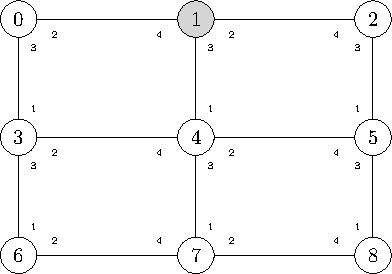
\includegraphics[keepaspectratio,width=0.7\textwidth,height=0.3\textheight]{chapters/nmp/images/3by3gridgraph.pdf}
    \caption[Basic 3×3 grid graph used for the example]{Basic 3×3 grid graph used for the example.  This example will focus on the perspective of node 1.  Other nodes are assumed to work equivalently, but their evolution is not discussed.  Nodes are labelled internally with their ID in the system (\(\iota\) in \cref{fig:nmp:iota_proxels_environment_oracle}), and each intermediary channel with the identity assigned to it by the nearby \gls{pe}.}
    \label{fig:nmp:basicgrid}
\end{figure}

Embodying the unknown processes of the oracle, the data for the received \(v\) terms have been randomly generated for this example and have no particular significance.

To supply a partial demonstration of the expected operation of the rule(s) which would replace the oracle, we compute the contents of outgoing messages according to the following simple rule: \cpruleinline{\cprulenonum{s_4}{\cprecv{\cpvw{W}{G}{\cpfunc{d}{A} \; \cpfunc{d}{B}}}{\iota}}{1}{s_5}{\cpsend{\cpvw{W}{G}{AB}}{\iota}}}  This rule merely sums the data received, and returns the newly computed outgoing message to the relevant node.

\setcounter{traces}{-1}

The total trace for this example is: \tracn{{\label{trace:nmp:0}}--}{--}{--} \tarr{} \tracn{\label{trace:nmp:1}0?*}{0?*}{0?*} \tarr{} \tracn{\label{trace:nmp:2}1?*}{0}{1?} \tarr{} \tracn{\label{trace:nmp:3}1}{0}{2?} \tarr{} \tracn{\label{trace:nmp:4}2?}{1?**}{2} \tarr{} \tracn{\label{trace:nmp:5}2}{2?}{2} \tarr{} \tracn{\label{trace:nmp:6}--}{--}{--}.  Each round number of the trace corresponds to the same row in \cref{tab:nmp:exampleobjects}, reflecting the state of node 1 at the end of that round.  Where the contents of a functor change, the functor and its changed contents are written in boldface to highlight the modifications.

\begin{table}
\setlength\extrarowheight{1ex}
\centering
\begin{tabular}{|l|l|}
\hline
\textbf{Round number} & \textbf{Objects in Node 1} \\ \hline
0 & \(\cpfunc{a}{\cpfunc{n}{2} \, \cpfunc{n}{3} \, \cpfunc{n}{4}}\) \\ \hline
1 & \(\cpfunc{a}{\cpfunc{n}{2} \, \cpfunc{n}{3} \, \cpfunc{n}{4}} \quad \cpfunc{\mathbf{i}}{\mathbf{2}} \quad \cpvvbf{\mathbf{2}}{\mathbf{0}}{\mathbf{1}} \; \cpvvbf{\mathbf{3}}{\mathbf{0}}{\mathbf{4}} \; \cpvvbf{\mathbf{4}}{\mathbf{0}}{\mathbf{7}}\) \\ \hline
2 & \(\cpfunc{a}{\cpfunc{n}{2} \, \cpfunc{n}{3} \, \cpfunc{n}{4}} \quad \cpfunc{i}{2} \quad \cpvvbf{2}{\mathbf{1}}{\mathbf{9}} \; \cpvv{3}{0}{4} \; \cpvvbf{4}{\mathbf{1}}{\mathbf{5}}\)  \\ \hline
3 & \(\cpfunc{a}{\cpfunc{n}{2} \, \cpfunc{n}{3} \, \cpfunc{n}{4}} \quad \cpfunc{i}{2} \quad \cpvv{2}{1}{9} \; \cpvv{3}{0}{4} \; \cpvvbf{4}{\mathbf{2}}{\mathbf{2}}\)  \\ \hline
4 & \(\cpfunc{a}{\cpfunc{n}{2} \, \cpfunc{n}{3} \, \cpfunc{n}{4}} \quad \cpfunc{i}{2} \quad \cpvvbf{2}{\mathbf{2}}{\mathbf{8}} \; \cpvvbf{3}{\mathbf{1}}{\mathbf{3}} \; \cpvv{4}{2}{2}\)  \\ \hline
5 & \(\cpfunc{a}{\cpfunc{n}{2} \, \cpfunc{n}{3} \, \cpfunc{n}{4}} \quad \cpfunc{i}{2} \quad \cpvv{2}{2}{8} \; \cpvvbf{3}{\mathbf{2}}{\mathbf{7}} \; \cpvv{4}{2}{2}\)  \\ \hline
6 & \(\cpfunc{a}{\cpfunc{n}{2} \, \cpfunc{n}{3} \, \cpfunc{n}{4}} \quad \cpfunc{i}{2}\)  \\ \hline
\end{tabular}
\caption[Objects present inside Node 1 at the end of each round]{Objects present inside Node 1 at the end of each round in the example}
\label{tab:nmp:exampleobjects}
\end{table}

\paragraph{Round One}
This round is where node 1 receives its inputs from the environment by rules 1 and 2.  The maximum message generations counter, and the messages with the initial data for the \gls{pe} come through the channel connected to the environment.  Node 1 starts this round holding only its adjacency list, in this case \(\cpfunc{a}{\cpfunc{n}{2} \, \cpfunc{n}{3} \, \cpfunc{n}{4}}\).

The receipt of messages for all three neighbours causes rule 3 to apply and node 1 to enter the sending cycle.  Two new \gls{oq} \(w\) messages are generated relating to each neighbour (because the other two neighbours will take the place of \(Y\) in applications of rule 3a --- recall that there is no \(Z\) in the rule for this node, as it only has three neighbours).  Rule 5 eliminates these duplicates, however, leaving one copy of each message for rule 6 to send to the oracle.  These outgoing messages to the oracle are \(\cpvw{2}{1}{\cpfunc{d}{4} \, \cpfunc{d}{7}}\), \(\cpvw{3}{1}{\cpfunc{d}{1} \, \cpfunc{d}{7}}\) and \(\cpvw{4}{1}{\cpfunc{d}{1} \, \cpfunc{d}{4}}\) for neighbours 2, 3, and 4, respectively.

Node 1 then enters a `blocking wait' (see \cref{sec:cps:blocking}) and remains inactive until the oracle returns the new \gls{nm} messages to send to each neighbour.  Rule 7 sees node 1 receive those messages and then immediately forward them to the neighbours.  The messages are not stored inside node 1 at the end of a step.  Following the example oracle rule described above, the messages sent are \(\cpvv{2}{1}{11}\), \(\cpvv{3}{1}{8}\) and \(\cpvv{4}{1}{5}\) for neighbours 2, 3, and 4, respectively.

The application of rule 7 brings the sending cycle to a close, and node 1 moves to state \(s_5\).  In this state, rule 8 clears away any receipt tokens present in the \gls{pe} and then moves to the termination check of rule 9.  At this point, none of the \(v\) messages hold generation counters equal to the maximum generation count, and so processing will continue.  Finally, node 1 proceeds with another blocking wait, until messages arrive from one or more of its neighbours.

\paragraph{Round Two}
The second round proceeds similarly to the first, but with two key differences.  Firstly, the incoming messages are received from neighbouring \glspl{pe} via the channels connecting node 1 to them.  Secondly, messages are received only from neighbours 2 and 4.  This generates receipt tokens for those neighbours and sees node 1 enter a new sending cycle.

The presence of receipt tokens for both neighbours 2 and 4 leads to the creation of two duplicate \(w\) \gls{oq} messages about neighbour 3.  In effect, 1 and 3 swap roles as \(X\) and \(Y\) in rule 3.  Again, rule 5 eliminates the duplicate, and the single message \(\cpvw{3}{2}{\cpfunc{d}{9} \, \cpfunc{d}{5}}\) is sent to the oracle with rule 6.  In turn, by rule 7, node 1 receives back \(\cpvv{3}{2}{14}\) and forwards it to neighbour 3, completing the sending cycle.  This is also the final message sent to neighbour 3, given that the maximum generation count for this system is two.

As before, node 1 moves from sending to clearing receipt tokens, checking whether it has completed \gls{nm}, and finally becomes quiescent once more, awaiting further messages from neighbours.

\paragraph{Round Three}
Round three begins with receiving a single message, the final message to be received from neighbour 4.  Unlike the earlier rounds, no new messages are sent out due to said receipt.  Neighbour 4 was already one of the neighbours with the highest generation count amongst the messages stored in node 1, and so while it can serve as \(X\) in rule 3, neither of neighbours 2 or 3 can serve as \(Y\) because their generation counts are lower than neighbour 4's.

The fact that rule 3 does \emph{not} apply means that rule 4 \emph{is} applied --- for the first time in this system's evolution.  Rule 4 unconditionally transitions node 1 back to removing all extant receipt tokens, before progressing to the termination check and then returning to awaiting new messages.

\paragraph{Round Four}
This time, neighbour 2 sends its final message, and neighbour 3, at last, sends its first message.  The receipt from neighbour 3 leads to two new single instances of messages relating to neighbours 2 and 4.  The receipt from neighbour 2 could ordinarily lead to another message to be sent to neighbour 3, as it would pair up with neighbour 4 to act as \(X\) and \(Y\), respectively, in rule 3.  This does not occur, however, as neighbour 2 (and 3) has reached the maximum generation count, so rule 3 is no longer applicable for it.

The messages to go to the oracle due to the receipt from neighbour 3 are \(\cpvw{2}{2}{\cpfunc{d}{3} \, \cpfunc{d}{2}}\) and \(\cpvw{4}{2}{\cpfunc{d}{8} \, \cpfunc{d}{3}}\).  Thus, the messages returned by the oracle and sent to neighbour 2 and are \(\cpvv{2}{2}{5}\) and \(\cpvv{4}{2}{11}\).  These are, the last two messages to be sent by node 1 to its neighbours.

\paragraph{Round Five}
Only one more message is still to be received, from neighbour 3 specifically. Node 1 will wait until said message is received, but at that point, all message generation counters will be equal to the maximum, and thus no further messages will be sent out to the neighbours.

Following the application of rule 10 to receive the final message from neighbour 3, node 1 returns to state \(s_2\) and the rules are again explored in top-down order.  This time, rule 3 is inapplicable, so rule 4 is applied, transitioning node 1 to state \(s_5\).  Rule 4 is the only rule applied at this step because it is the only rule which moves from state \(s_2\) to state \(s_5\).  Next, rule 8 deletes the last receipt token.  Again, rule 8 is the only rule applied because it is the only one to feature its state transitions.  Finally, without any \(v\) messages with a generation count below the maximum present in the \gls{pe}, by rule 9, node 1 moves to state \(s_7\) and the finalisation phase.

\paragraph{Round Six}
Round six is the final round of the evolution of the system, for node 1 at least.  With node 1 in state \(s_7\), the only applicable rule is rule 11.  The effect of rule 11 is to send every \(v\) message stored in node 1 to the oracle, renaming them to \(w'\) messages so that the oracle recognises them as finalisation messages rather than \gls{oq} messages for \gls{nm} purposes.

Eventually, the oracle will return the final result message, with the contained datum computed by some means from the messages the oracle received from node 1.  That message is immediately forwarded back to the environment, and evolution of node 1 halts.  Once all other nodes have halted, evolution of the system will have terminated.
\section{\label{sec:nmp:analysis}Asynchronous System Analysis}

This \lcnamecref{sec:nmp:analysis} examines and analyses the asynchronous \gls{pe}-specific system of \cref{sec:nmp:pespecific}.  Firstly, it describes and proves several properties about the system, in particular, that the asynchronous system exchanges precisely the same number of \gls{nm} messages as the \gls{gs} system of \cref{sec:nmp:systemwide}.  Then, it states three conjectures about the system, yet to be proven or disproven mathematically, before examining the asynchronous system's complexity from the standpoint of the rules and symbols used.  Lastly, the \lcnamecref{sec:nmp:analysis} discusses some visualisations of the propagation of ``influence'' from one \gls{pe} in a \gls{fne} grid to others, over multiple steps.

Recall that the fundamental difference in behaviour between the \gls{gs}, \gls{ls} and asynchronous variants is the timing of when they send out new messages relating to when they have received messages for the previous generation.  Under the \gls{gs} approach, \emph{every} \gls{pe} waits until every other \gls{pe} has received all incoming messages before progressing.  Following the \gls{ls} methodology, each \gls{pe} waits until it has received all of its due incoming messages before proceeding, \emph{but without regard} to any other \gls{pe}.  Lastly, for the asynchronous variant, a \gls{pe} waits only until it has received the \(n - 1\) required messages from the other neighbours of generation \(g\) before sending the appropriate generation \(g + 1\) message to the \(n^\text{th}\) neighbour.

\subsection{\label{sec:nmp:msgprops}Messaging Properties and Behaviours}

Consider a cell (\gls{pe}) $\pi_0$ in the asynchronous framework of \cref{sec:nmp:pespecific},
where the maximum generation count is $I$, set by the environment via $\cpfunc{i}{I}$.
Without loss of generality, 
we consider only a \gls{fne} system and
assume that $\pi_0$ is a non-border/non-corner cell with four neighbours, 
$\pi_k$, accessible via channels labelled by $k \in \{ 1, 2, 3, 4 \}$. 

\begin{lemma}\label{lemma:nmp:-0}
    For any $k \in \{ 1, 2, 3, 4 \}$, after each round except the last,
    cell $\pi_0$ contains exactly one $k$-tagged value $\cpvv{k}{\cpdiscard}{\cpdiscard}$, 
    which is accepted from channel $k$ 
    --- except the first round, when that value $v$ comes from the environment channel $e$.
\end{lemma}

\begin{proof}
    By \cpruleref{rule:nmp:proxspec:recvinputs}, cell $\pi_0$ starts by accepting a value $\cpvv{k}{0}{\cpdiscard}$, from the environment channel $e$.
    \cpRuleref{rule:nmp:proxspec:recvfromneighs} gives the only possibility of obtaining another $k$-tagged value, by replacing the current value $v$ with another value $v'$, accepted from channel $k$.
\end{proof}

\begin{remark}
    In fact, \cref{lemma:nmp:-0} holds practically at all times, not just at the end of each round.  The only exceptions are: before the start of the system's evolution and application of \cpruleref{rule:nmp:proxspec:recvinputs}; and after the start of the finalisation phase, specifically after applying \cpruleref{rule:nmp:proxspec:finaloracle}.
\end{remark}

\begin{lemma}\label{lemma:nmp:-1}
    For any $k \in \{ 1, 2, 3, 4 \}$, the time sequence of generation numbers $g \geq 0$ of accepted values $\cpvv{k}{g}{\cpdiscard}$ forms an arithmetic progression with step size one.
\end{lemma}

\begin{proof}
    Proof by induction. Cell $\pi_0$ starts with value $\cpvv{k}{0}{\cpdiscard}$, received via the environment channel $e$.
    Assume that this hypothesis holds for a given $g \geq 0$, appearing as a generation number in value $\cpvv{k}{g}{\cpdiscard}$. \cpRuleref{rule:nmp:proxspec:recvfromneighs} gives the only possibility of changing this number, by replacing the current value with another $v$ value, where the generation number is strictly greater by one, 
    $\cpvv{k}{g+1}{\cpdiscard}$.
\end{proof}

\begin{remark}\label{remark:nmp:-1}
The conclusion of \cref{lemma:nmp:-1} will hold even in the hypothetical case that cell $\pi_k$ would be allowed to send multiple copies of the same message $v$. 
Only the first received copy will be accepted, and the rest will be ignored,
courtesy of \cpruleref{rule:nmp:proxspec:recvfromneighs}. However, this is not the case, as excess \(w\) \gls{oq} messages are deleted by \cpruleref{rule:nmp:proxspec:uniq}. 
\end{remark}

\begin{lemma}\label{lemma:nmp:-2}
    For any $k \in \{ 1, 2, 3, 4 \}$, if channels are reliable and cell $\pi_k$ sends a sequence of messages that reach $\pi_0$ as $\cpvv{k}{g}{\cpdiscard}$, $g \in [1,I]$, 
    then $\pi_0$ accepts all these values in the order of their increasing generation numbers.
\end{lemma}

\begin{proof}
    Channels are reliable, so no message is lost. Channels in \gls{cps} are not inherently FIFO, but cell $\pi_0$ will still pick messages with increasing generation numbers, by \cref{lemma:nmp:-1}.
    As defined by the async version of the model, any messages arriving out-of-order are not lost, but stored in a multiset at the end of the channel
    and will be picked when their time comes.
\end{proof}

\begin{lemma}\label{lemma:nmp:-3}
    For any $k \in \{ 1, 2, 3, 4 \}$, and $g \in [1, I]$: cell $\pi_0$ sends one generation $g$ value $v$ over channel $k$, if and only if $\pi_0$ has received three generation $g-1$ values $v$ from three distinct channels $k' \in 
    \{ 1, 2, 3, 4 \} \setminus \{ k \}$.
\end{lemma}

\begin{proof}
    \textbf{Only if}. Assume that $\pi_0$ sends out a generation $g$ message $v$ over channel $k$.   
    This may only happen by \cpruleref{rule:nmp:proxspec:recvfromoracle}, where $\pi_0$ just forwards the same message $v$, received as $w$ from its oracle. 
    \cpRuleref{rule:nmp:proxspec:sendtooracle} triggers the oracle to build this message $w$, based on three other $v$ messages 
    $\cpvv{k_1}{g_1}{d_1}$, $\cpvv{k_2}{g_2}{d_2}$, $\cpvv{k_3}{g_3}{d_3}$, 
    where $g_1 = g-1$, $g_2, g_3 \geq g_1$, and $k, k_1, k_2, k_3$ are all distinct.
    By \cref{lemma:nmp:-2}, $\pi_0$ must have also received two generation $g-1$ values $v$, from $k_2$ and $k_3$.
    Thus, cell $\pi_0$ has received three values $\cpvv{k_1}{g-1}{d_1}$, $\cpvv{k_2}{g-1}{\cpdiscard}$, $\cpvv{k_3}{g-1}{\cpdiscard}$.
    
    \textbf{If}. Assume that $\pi_0$ accepts three values $\cpvv{k_1}{g'}{d_1}$, $\cpvv{k_2}{g'}{\cpdiscard}$, $\cpvv{k_3}{g'}{\cpdiscard}$, where $g' = g - 1 \geq 0$. These values need not arrive at the same round. Without loss of generality, assume that $\pi_0$ has just received the first value, $\cpvv{k_1}{g'}{d_1}$, while the other values may have been received and even updated already, 
    $\cpvv{k_2}{g'+h_2}{d_2}$, $\cpvv{k_3}{g'+h_3}{d_3}$, $h_2, h_3 \geq 0$.
    \cpRuleref{rule:nmp:proxspec:makews} applies and creates at least two identical \(w\) messages $\cpvw{k_4}{g' + 1}{d}$, where \(d = \cpfunc{d}{d_1}, \, \cpfunc{d}{d_2}, \, \cpfunc{d}{d_3}\). Additional $w$ messages may be created, if either $h_2=0$, or $h_3=0$, or both. This doesn't matter, 
    as excess \(w\) messages are deleted by \cpruleref{rule:nmp:proxspec:uniq}, so only one $\cpvw{k_4}{g' + 1}{d}$ remains.
    This message goes to the oracle, 
    which creates and returns the value $\cpvw{k_4}{g'+1}{d'} = \cpvv{k_4}{g}{d'}$, 
    further forwarded by \cpruleref{rule:nmp:proxspec:recvfromoracle} to $\pi_{k_4}$, over channel $k_4$.
\end{proof}

\begin{remark}
    The behaviour of Lemma~\ref{lemma:nmp:-3} is also true for the \gls{gs} and \gls{ls} variants too.  The key difference for the asynchronous variant is that the new outgoing message for generation \(g\) is sent as soon as possible after those three messages for generation \(g - 1\) have been received, whereas the other two variants will await receipt of the final also message before sending any new ones.
\end{remark}

\begin{theorem}\label{theorem:nmp:-1}
    For each $k \in \{ 1, 2, 3, 4 \}$, and each $g \in [0, I]$:
    \begin{inparaenum}[(i)]
        \item\label{enumitem:nmp:analysis:-1:1} $\pi_0$ receives one $k$-tagged generation $g$ value $v$; and
        \item\label{enumitem:nmp:analysis:-1:2} if $g < I$, $\pi_0$ sends one $k$-tagged generation $g+1$ value $v$.
    \end{inparaenum}
\end{theorem}

\begin{proof}
By bounded induction on $g$. Base case: $g = 0$. By \cpruleref{rule:nmp:proxspec:recvinputs}, cell $\pi_0$ receives \emph{four} $k$-tagged generation $g$ values -- one for each $k \in \{ 1, 2, 3, 4 \}$ -- from the environment channel $e$ (acting on behalf of its neighbour channels). By \cref{lemma:nmp:-3}, applied \emph{four} times, $\pi_0$ sends out \emph{four} generation $g+1$ values $v$, one over each channel $k$.

Induction step: assume that the induction hypothesis holds for 
$g \in [0, I)$, and we prove that it still holds for $g+1$.
The induction hypothesis holds for all cells, 
including $\pi_0$ and $\pi_k$. 
% Thus, by part (ii), each cell $\pi_k$ sends a generation $g+1$ value $v$,
Thus, by part (\ref{enumitem:nmp:analysis:-1:2}), each cell $\pi_k$ sends a generation $g+1$ value $v$, 
which is further received by $\pi_0$, as $\cpvv{k}{g+1}{\cpdiscard}$.
This proves part (\ref{enumitem:nmp:analysis:-1:1}) of the induction step.

If $g+1 < I$, rule 9 does not apply and, 
as shown by \cref{lemma:nmp:-3}, applied \emph{four} times, 
$\pi_0$ sends out \emph{four} generation $g+2$ values $v$, one over each channel $k$.
This proves part (\ref{enumitem:nmp:analysis:-1:2}) of the hypothesis.
\end{proof}

\begin{theorem}\label{theorem:nmp:-2}
    Cell (\gls{pe}) \(\pi_0\) does not send any message to its neighbours at generation \(g > I\).
\end{theorem}

\begin{proof}
    \Gls{oq} \(w\) messages (and thus indirectly \gls{nm} \(v\) messages) are created only by \cpruleref{rule:nmp:proxspec:makews}, with generation counts \(g + 1\), only if \(g + 1 \leq I\).  The promoter \(\cpfunc{i}{G1\cpdiscard}\) for \cpruleref{rule:nmp:proxspec:makews} prevents the creation of any \(w\) message with a larger generation count.
\end{proof}

\begin{theorem}\label{theorem:nmp:-3}
    For each cell $\pi_0$, the neighbourhood (inter-cell) messaging loop stops after receiving the last generation $I$ value.
\end{theorem}

\begin{proof}
    After receiving the last generation \(I\) message, \cpruleref{rule:nmp:proxspec:makews} does not apply (per \cref{theorem:nmp:-2}), and instead control flows by \cpruleref{rule:nmp:proxspec:skiptorecv} to state \(s_5\), then to \(s_6\) by \cpruleref{rule:nmp:proxspec:clearrs}.  Finally, \cpruleref{rule:nmp:proxspec:movetoend} applies, and the control flow breaks out of the main messaging loop, proceeding to state \(s_7\) and the finalisation phase, where no further \gls{nm} occurs. 
\end{proof}

\begin{theorem}\label{theorem:nmp:-4}
    For the asynchronous system in \cref{sec:nmp:pespecific}, 
    each cell (\gls{pe}) sends and receives the same number of messages as in the \gls{gs} system in \cref{sec:nmp:systemwide} and the \gls{ls} system in \cref{sec:nmp:localsync}.   
    Thus, the system as a whole uses the same number of messages.
\end{theorem}

\begin{proof}
    Direct consequence of \cref{theorem:nmp:-1,theorem:nmp:-3}
\end{proof}

\begin{remark}\label{remark:nmp:-2}
    The evolution of the asynchronous version can be suggestively summarised by
    analysing the following four typical cases of cell $\pi_0$ snapshots,
    which focus on the received values having the \emph{least generation number}, here indicated by $g$.
    Note that each star (*) indicates the channel of the incoming value 
    that triggers the sending of a generation $g+1$ message, 
    \emph{not} the channel over which this is sent.
    Without loss of generality, in the case of confluent non-determinism,
    stars are allocated to the first possible choice (for illustrative purposes).
    
    \begin{enumerate}
    \item $(g?***, g?*, g?, g?)$: 
    $\pi_0$ receives all \emph{four} generation $g$ values in the same round, by \cpruleref{rule:nmp:proxspec:recvfromneighs}. 
    As shown by \cref{lemma:nmp:-3}, applied \emph{four} times, 
    $\pi_0$ sends \emph{four} generation $g+1$ values.
    \cpRuleref{rule:nmp:proxspec:makews} will initially create \emph{six} \gls{oq} messages per neighbour (for a total of 24)
    but the excess ones will be deleted, so exactly one \(w\) message per channel will remain and be sent to the oracle.
    
    \medskip
    \item $(g?***, g?*, g?, g_4)$, $g < g_4$: 
    $\pi_0$ receives \emph{three} generation $g$ values in the same round, by \cpruleref{rule:nmp:proxspec:recvfromneighs}.
    The fourth value is at least one generation ahead.    
    This case evolves similarly to case (1) above, with a few changes in the details.
    As shown by \cref{lemma:nmp:-3}, still applied \emph{four} times, 
    $\pi_0$ sends \emph{four} generation $g+1$ values.
    The rules will create \emph{four} \gls{oq} messages for each of the first three channels,
    and \emph{six} \gls{oq} messages for the last channel (for a total of 18),
    but the excess ones will be deleted, so exactly one \gls{oq} message per channel will remain and be sent.
    
    \medskip
    \item $(g?***, g?*, g_3, g_4)$, $g < g_3, g_4$: 
    $\pi_0$ receives \emph{two} generation $g$ values in the same round, by \cpruleref{rule:nmp:proxspec:recvfromneighs}.
    The other two values are at least one generation ahead.    
    This case evolves similarly to case (2) above, with a few changes in the details.
    As shown by \cref{lemma:nmp:-3}, still applied \emph{four} times, 
    $\pi_0$ sends \emph{four} generation $g+1$ values.
    The rules will create \emph{two} \gls{oq} messages for each of the first two channels,
    and \emph{four} \gls{oq} messages for the last two channels (for a total of 12),
    but the excess ones will be deleted, so only one \gls{oq} message per channel will remain and be sent.
    
    \medskip
    \item $(g?***, g_2, g_3, g_4)$, $g < g_2, g_3, g_4$: 
    $\pi_0$ receives \emph{one} single generation $g$ value in a given round, by \cpruleref{rule:nmp:proxspec:recvfromneighs}.
    The last three values are at least one generation ahead.
    As shown by \cref{lemma:nmp:-3}, applied \emph{three} times, 
    $\pi_0$ sends \emph{three} generation $g+1$ values.
    The rules will create and use \emph{two} \gls{oq} messages for each of the last three channels (for a total of 6), but the excess ones will be deleted.
    
    \medskip
    The question arises: when will $\pi_0$ send its fourth generation $g+1$ value, over channel $1$? Brief answer: that message was already sent,
    before the current round!
    
    \medskip
    % Indeed, Lemmas~\ref{lemma:nmp:-1},\ref{lemma:nmp:-2} show that,
    Indeed, \cref{lemma:nmp:-1,lemma:nmp:-2} show that,
    from each channel $k \in \{ 2, 3, 4\}$, 
    $\pi_0$ has received, in order, 
    messages with generation numbers $g, g+1, \ldots, g_k$.
    Consider the round when $\pi_0$ receives the last such message for generation $g$. Without loss of generality, assume that this was from channel $2$.
    Thus, at that round, the summary snapshot was $(g_1, g?, g'_3, g'_4)$,
    with $g_1 < g \leq g'_3, g'_4$.
    By \cref{lemma:nmp:-3}, \emph{one} generation $g+1$ value was then sent over channel $1$.
    \end{enumerate}    
    
    Note also that, at the outset of cases (1,2,3), no other messages for generation $g+1$ will have been sent yet because too few messages at generation $g$ have been received. 
    These notes may be used to create alternate proofs of our main results.

\end{remark}

\subsection{Generational Confluence}
The asynchronous system is \emph{not} (necessarily) confluent.  Messages may be received in such an order that the contents of some messages might not be used in the preparation of new messages, since two messages potentially can be received from one neighbour between receipts from a different neighbour.  Nevertheless, for a \gls{pe} to send a message for generation \(g + 1\) to neighbour \(k\), it must have received messages for \emph{at least} generation \(g\) from all other neighbours.  Therefore, no input data will be `out-of-date'.  This concept is given the name \emph{generational confluence}.

\begin{conjecture}\label{conj:nmp:1}
A \gls{nmp} system following the asynchronous rules of \cref{sec:nmp:pespecific} will be \emph{approximately/generationally} confluent.  Under a wide variety of practical conditions (\eg{} when the base synchronous version is convergent), every evolution of the system will produce a similar result, no matter the specific ordering of the messaging.
\end{conjecture}

\begin{conjecture}\label{conj:nmp:2}
    The asynchronous behaviour, specifically the potential for \glspl{pe} to forgo the use of data from particular messages in favour of newer data, will lead to a final output that is no worse than the synchronous variants' and might result in a `better quality' result, for a particular domain-specific meaning of quality.
\end{conjecture}

Determining the truth or falsity of \cref{conj:nmp:1,conj:nmp:2} is still an open problem requiring further study (but see \cref{sec:nmp:convergence}).  Ideally, one would also clarify and quantify what ``similar'' means in this context.

\begin{proposition}\label{prop:nmp:3}
    No matter the approach to \gls{nmp} employed, the most generations any given \gls{pe} may be ahead of any other \gls{pe} on the lattice depends on their distance from each other, as measured by the smallest number of intermediate \glspl{pe} along any path between the two.
\end{proposition}

The requirement for a \gls{pe} to have received messages from every other neighbour before preparing a message to send to the final neighbour means that, at a certain point, a \gls{pe} transitively depends on its neighbours' neighbours in an ever-expanding radius.  A given \gls{pe} cannot send a new message to neighbour 4 until it has received messages from neighbours 1-3.  In turn, neighbour 4 cannot send messages to any of its other neighbours besides the original \gls{pe} until it has received the next message from the original \gls{pe}.  The same then applies to those neighbours of the original \gls{pe}'s neighbour 4, \etc{}.

This reasoning gives rise to the intuition in \cref{prop:nmp:3}.  If one of the \glspl{pe} stops sending messages but has not yet reached its maximum generation, the neighbouring \glspl{pe} will successively be unable to send further messages themselves, which will ripple across the lattice and eventually prevent farther \glspl{pe} from sending further messages as well.  Until the ripple has progressed across the lattice, however, the more remote \glspl{pe} may still send new messages.  Therefore, in all cases where two \glspl{pe} have a path between them, there is an inter-dependency, albeit in some cases far removed.  As yet, no suitable and convincing formal proof of this idea has been found.

\subsection{Rule and Symbol Complexity}
Overall, the rule and symbol complexity of the system is relatively low, but given that some elements of any specific \gls{nmp} process are abstracted away (\eg{} the oracle), this is likely an underestimate for a given final implementation.

\subsubsection{Rule Complexity}
The total system requires 12 rules.  Two for the initialisation phase, eight for the joint \gls{nm} \& \gls{oq} phases -- only two directly involve interaction with the oracle, but others prepare for said interaction -- and two for the finalisation phase.  The two rules that involve direct interaction with the oracle, rules \cpruleref*{rule:nmp:proxspec:sendtooracle} and \cpruleref*{rule:nmp:proxspec:recvfromoracle}, will normally be replaced with an arbitrary new \gls{ruleset}, however.  Thus, it can be said that there are 10 rules relating to the structure and process for \gls{nmp}, and two stub rules which stand in for a more complex process.

\subsubsection{Symbol Complexity}
Across all 12 rules, three atoms, eight functors, and nine states are used.  This gives a total symbol complexity of 20 distinct symbols.  As with the rule complexity, there likely will be more symbols used when the \gls{oq} phase is expanded to encompass a desired computation process.

\subsection{Visualisations}
Sequences of visualisations of the evolution of a sample \gls{fne} system have been created to explore the messaging behaviour of \gls{nmp}.  These sequences reflect the changes on a small grid that result from \gls{nmp} following \cref{sec:nmp:pespecific}'s system.  Each square on a grid represents one \gls{pe}, and the \glspl{pe} are assumed to be connected in the standard \gls{fne} manner.

Each sequence was generated using a script by computing values over the grid at the end of each round of messaging and writing the results out to a standalone .tex file, then compiling the .tex file to produce an output .pdf.  In each case, the grid starts with all zero values, except for the centre \gls{pe}, which starts with a `full-strength' value --- represented by wholly white and completely black squares, respectively.  The value to display at a given grid point for each round was in turn computed by selecting the maximum from among the data stored in the corresponding \gls{pe}.

Each of the sequences uses a different method for computing the values present in a given square, and so depicts a different aspect of the spread of the `influence' of the initial data in the centre \gls{pe}.  The approach used here was effectively the \gls{ls} variant, but the results apply equally to the variants.

\subsubsection{Maximum Over Messages Received and Internal Datum}
\begin{figure}
    \centering
    \subcaptionbox{Round 0}{
\includegraphics[width=0.19\textwidth]{chapters/nmp/images/grids/maxpdatum/nodelay/maxWithPDatum_no_delays_four_generations_round_0.pdf}}
    \subcaptionbox{Round 1}{
\includegraphics[width=0.19\textwidth]{chapters/nmp/images/grids/maxpdatum/nodelay/maxWithPDatum_no_delays_four_generations_round_1.pdf}}
    \subcaptionbox{Round 2}{
\includegraphics[width=0.19\textwidth]{chapters/nmp/images/grids/maxpdatum/nodelay/maxWithPDatum_no_delays_four_generations_round_2.pdf}}
    \subcaptionbox{Round 3}{
\includegraphics[width=0.19\textwidth]{chapters/nmp/images/grids/maxpdatum/nodelay/maxWithPDatum_no_delays_four_generations_round_3.pdf}}
    \subcaptionbox{Round 4}{
\includegraphics[width=0.19\textwidth]{chapters/nmp/images/grids/maxpdatum/nodelay/maxWithPDatum_no_delays_four_generations_round_4.pdf}}
    \caption[Visualisation of the spread of `influence' from the centre \glsxtrshort{pe} during \glsxtrlong{nmp}]{Visualisation of the spread of `influence' from the centre \gls{pe} during \gls{nmp}.  Each square's value was computed as the maximum over both the last messages received, and a datum stored by the \gls{pe}}
    \label{fig:nmp:maxpdatum}
\end{figure}

The sequence in \cref{fig:nmp:maxpdatum} was produced by using the maximum of the \gls{pe}'s current messages received from the other neighbours \emph{and} a separate value stored internally and updated when computing the new outgoing messages.  The extra value was updated at each step to be the maximum of itself or the messages currently held.  The net effect of this was to ensure that when a message carrying information from the centre \gls{pe} arrived, the current \gls{pe} would turn black and remain that way.  \Cref{fig:nmp:maxpdatum} shows that this information propagates outwards as expected, given the nature of the updates.

\begin{figure}
    \centering
    \subcaptionbox{Round 0}{
\includegraphics[width=0.19\textwidth]{chapters/nmp/images/grids/maxpdatum/delay2/maxWithPDatum_delay2_four_generations_round_0.pdf}}
    \subcaptionbox{Round 1}{
\includegraphics[width=0.19\textwidth]{chapters/nmp/images/grids/maxpdatum/delay2/maxWithPDatum_delay2_four_generations_round_1.pdf}}
    \subcaptionbox{Round 2}{
\includegraphics[width=0.19\textwidth]{chapters/nmp/images/grids/maxpdatum/delay2/maxWithPDatum_delay2_four_generations_round_2.pdf}}
    \subcaptionbox{Round 3}{
\includegraphics[width=0.19\textwidth]{chapters/nmp/images/grids/maxpdatum/delay2/maxWithPDatum_delay2_four_generations_round_3.pdf}}
    \subcaptionbox{Round 4}{
\includegraphics[width=0.19\textwidth]{chapters/nmp/images/grids/maxpdatum/delay2/maxWithPDatum_delay2_four_generations_round_4.pdf}}
    \subcaptionbox{Round 5}{
\includegraphics[width=0.19\textwidth]{chapters/nmp/images/grids/maxpdatum/delay2/maxWithPDatum_delay2_four_generations_round_5.pdf}}
    \subcaptionbox{Round 6}{
\includegraphics[width=0.19\textwidth]{chapters/nmp/images/grids/maxpdatum/delay2/maxWithPDatum_delay2_four_generations_round_6.pdf}}
    \subcaptionbox{Round 7}{
\includegraphics[width=0.19\textwidth]{chapters/nmp/images/grids/maxpdatum/delay2/maxWithPDatum_delay2_four_generations_round_7.pdf}}
    \subcaptionbox{Round 8}{
\includegraphics[width=0.19\textwidth]{chapters/nmp/images/grids/maxpdatum/delay2/maxWithPDatum_delay2_four_generations_round_8.pdf}}
    \subcaptionbox{Round 9}{
\includegraphics[width=0.19\textwidth]{chapters/nmp/images/grids/maxpdatum/delay2/maxWithPDatum_delay2_four_generations_round_9.pdf}}
    \caption[Visualisation of the spread of `influence' from the centre \glsxtrshort{pe} during \glsxtrlong{nmp}]{Visualisation of the spread of `influence' from the centre \gls{pe} during \gls{nmp}.  Each square's value was computed as the maximum over both the last messages received, and a datum stored by the \gls{pe}, and with delivery delays of two rounds on messages going to the neighbours below and to the left}
    \label{fig:nmp:maxpdatumdelays}
\end{figure}

More interesting is \cref{fig:nmp:maxpdatumdelays}.  The same update computations were performed, but a two-round delay was introduced for the delivery of messages to the neighbours below and to the left of the sending \gls{pe}.  Messages destined for the neighbours to the right and above of the sending \gls{pe} were delivered without delays, as in \cref{fig:nmp:maxpdatum}.  The eventual symmetry of the shape may seem surprising at first, but is actually logical.  Remember that every \gls{pe}/square on the grid is a neighbour of the ones to the top and right, and will only receive messages from those neighbours after the two-round delay --- which consequently means that they in turn only send out messages to their bottom and left \emph{after} that delay.  See also \cref{prop:nmp:3}.

What might happen if there is a systematic delay in only one direction, and thus potentially messages from all other neighbours might arrive relatively quickly?  This is examined in \cref{fig:nmp:maxpdatumdelayswestonly}, where a two round delay was introduced for messages sent to the left only.  In this case, the overall shape of the \glspl{pe} on the grid who have received a message containing `influence' from the centre \gls{pe} still invariably ends up returning to a symmetrical, balanced shape.  It is a different shape, however, from that seen in \cref{fig:nmp:maxpdatum,fig:nmp:maxpdatumdelays}, and is not centred on the centre \gls{pe}.  Instead, it grows with a bias towards the right.%  This eventual symmetry may appear surprising at first, but is to be expected for similar reasons to the basis for \autoref{prop:3}.  A \gls{pe} can only send a message to a neighbour once it has received the messages from the other neighbours, and this dependency is (effectively) transitive.  Thus, if some messages take much longer to arrive, \glspl{pe} will end up being forced to wait for them, directly or indirectly.

\begin{figure}
    \centering
    \subcaptionbox{Round 0}{
\includegraphics[width=0.19\textwidth]{chapters/nmp/images/grids/maxpdatum/delay2westonly/maxWithPDatum_delay2_west_only_four_generations_round_0.pdf}}
    \subcaptionbox{Round 1}{
\includegraphics[width=0.19\textwidth]{chapters/nmp/images/grids/maxpdatum/delay2westonly/maxWithPDatum_delay2_west_only_four_generations_round_1.pdf}}
    \subcaptionbox{Round 2}{
\includegraphics[width=0.19\textwidth]{chapters/nmp/images/grids/maxpdatum/delay2westonly/maxWithPDatum_delay2_west_only_four_generations_round_2.pdf}}
    \subcaptionbox{Round 3}{
\includegraphics[width=0.19\textwidth]{chapters/nmp/images/grids/maxpdatum/delay2westonly/maxWithPDatum_delay2_west_only_four_generations_round_3.pdf}}
    \subcaptionbox{Round 4}{
\includegraphics[width=0.19\textwidth]{chapters/nmp/images/grids/maxpdatum/delay2westonly/maxWithPDatum_delay2_west_only_four_generations_round_4.pdf}}
    \subcaptionbox{Round 5}{
\includegraphics[width=0.19\textwidth]{chapters/nmp/images/grids/maxpdatum/delay2westonly/maxWithPDatum_delay2_west_only_four_generations_round_5.pdf}}
    \subcaptionbox{Round 6}{
\includegraphics[width=0.19\textwidth]{chapters/nmp/images/grids/maxpdatum/delay2westonly/maxWithPDatum_delay2_west_only_four_generations_round_6.pdf}}
    \subcaptionbox{Round 7}{
\includegraphics[width=0.19\textwidth]{chapters/nmp/images/grids/maxpdatum/delay2westonly/maxWithPDatum_delay2_west_only_four_generations_round_7.pdf}}
    \subcaptionbox{Round 8}{
\includegraphics[width=0.19\textwidth]{chapters/nmp/images/grids/maxpdatum/delay2westonly/maxWithPDatum_delay2_west_only_four_generations_round_8.pdf}}
    \subcaptionbox{Round 9}{
\includegraphics[width=0.19\textwidth]{chapters/nmp/images/grids/maxpdatum/delay2westonly/maxWithPDatum_delay2_west_only_four_generations_round_9.pdf}}
    \caption[Visualisation of the spread of `influence' from the centre \glsxtrshort{pe} during \glsxtrlong{nmp}.]{Visualisation of the spread of `influence' from the centre \gls{pe} during \gls{nmp}.  Each square's value was computed as the maximum over both the last messages received, and a datum stored by the \gls{pe}, and with delivery delays of two rounds on messages going to the left only}
    \label{fig:nmp:maxpdatumdelayswestonly}
\end{figure}

\subsubsection{Maximum Over Messages Received}
\begin{figure}
    \centering
    \subcaptionbox{Round 0}{
\includegraphics[width=0.19\textwidth]{chapters/nmp/images/grids/max/nodelay/max_no_delay_four_generations_round_0.pdf}}
    \subcaptionbox{Round 1}{
\includegraphics[width=0.19\textwidth]{chapters/nmp/images/grids/max/nodelay/max_no_delay_four_generations_round_1.pdf}}
    \subcaptionbox{Round 2}{
\includegraphics[width=0.19\textwidth]{chapters/nmp/images/grids/max/nodelay/max_no_delay_four_generations_round_2.pdf}}
    \subcaptionbox{Round 3}{
\includegraphics[width=0.19\textwidth]{chapters/nmp/images/grids/max/nodelay/max_no_delay_four_generations_round_3.pdf}}
    \subcaptionbox{Round 4}{
\includegraphics[width=0.19\textwidth]{chapters/nmp/images/grids/max/nodelay/max_no_delay_four_generations_round_4.pdf}}
    \caption[Visualisation of the spread of `influence' from the centre \glsxtrshort{pe} during \glsxtrlong{nmp}]{Visualisation of the spread of `influence' from the centre \gls{pe} during \gls{nmp}.  Each square's value was computed as the maximum over the last messages received}
    \label{fig:nmp:max}
\end{figure}

The sequence in \cref{fig:nmp:max} was produced by using the maximum of the messages received from the other neighbours when computing the new outgoing messages for each \gls{pe}.\footnote{Given that both systems only have two values for each cell and updates to a given cell are based on values in surrounding ones, it does not seem coincidental that this progression bears some resemblance to Conway's Game of Life.}  As with the sequence in \cref{fig:nmp:maxpdatum}, the spread of the influence from the centre \gls{pe} moves outward, similar to an expanding `+' shape.  Notably, however, points in the grid (except the centre \gls{pe} for one round) oscillate between the minimum and the maximum, showing that the influence from the centre \gls{pe} is only relevant for every second message update computation.  Felzenzswalb \& Huttenlocher \cite{Felzenszwalb2006} noticed this oscillating behaviour and used it to halve the number of computations required to produce the same results in their improved \gls{bp} \gls{sm} implementation.

\subsubsection{Mean Over Messages Received}
\begin{figure}
    \centering
    \subcaptionbox{Round 0}{
\includegraphics[width=0.19\textwidth]{chapters/nmp/images/grids/mean/nodelay/mean_no_delay_four_generations_round_0.pdf}}
    \subcaptionbox{Round 1}{
\includegraphics[width=0.19\textwidth]{chapters/nmp/images/grids/mean/nodelay/mean_no_delay_four_generations_round_1.pdf}}
    \subcaptionbox{Round 2}{
\includegraphics[width=0.19\textwidth]{chapters/nmp/images/grids/mean/nodelay/mean_no_delay_four_generations_round_2.pdf}}
    \subcaptionbox{Round 3}{
\includegraphics[width=0.19\textwidth]{chapters/nmp/images/grids/mean/nodelay/mean_no_delay_four_generations_round_3.pdf}}
    \subcaptionbox{Round 4}{
\includegraphics[width=0.19\textwidth]{chapters/nmp/images/grids/mean/nodelay/mean_no_delay_four_generations_round_4.pdf}}
    \caption[Visualisation of the spread of `influence' from the centre \glsxtrshort{pe} during \glsxtrlong{nmp}]{Visualisation of the spread of `influence' from the centre \gls{pe} during \gls{nmp}.  Each square's value was computed as the mean over the last messages received}
    \label{fig:nmp:mean}
\end{figure}

The sequence in \cref{fig:nmp:mean} was produced by using the mean of the messages received from the other neighbours when computing the new outgoing messages for each \gls{pe}.  This sequence makes it clear that as the initial information from a given \gls{pe} diffuses across the grid, its direct influence upon the data in the \glspl{pe} gradually dilutes.  After just four rounds of message passing, the `signal strength' from the centre \gls{pe} has become so weak as to be almost imperceptible in the most distant locations it has reached, \eg{} points (0,4) and (4,8), assuming a zero-based grid count beginning in the upper-left corner.
\section{\label{sec:nmp:experiments}Experimental Results}

This \namecref{sec:nmp:experiments} presents the results of a handful of small experiments with short prototype programs, performed to validate \cref{ruleset:nmp:proxspec} and investigate the properties of the \gls{pe}-specific approach to \gls{nmp}.  In particular, these experiments:
\begin{inparaenum}[(i)]
\item simulated the operation of the \gls{ruleset} without actually passing messages, to verify empirically that \cref{theorem:nmp:-4} holds for an arbitrary \gls{pe};
\item implemented and benchmarked three variants of the three \gls{nmp} variants operating on a \gls{fne} grid, to assess whether the fully asynchronous version genuinely completes faster on average;
\item investigated the variants' convergence behaviour;
\item compared the timings of the variants for when the first, `average' and last \gls{pe} finish their processing.
\end{inparaenum}
Source code for the described scripts or programs may be found at \url{https://github.com/jcoo092/NeighbourhoodMessagePassingExperiments}.

\subsection{Validation of Rules for Asynchronous Neighbourhood Message Passing}
A short script was written in \fsharp{}.  This script takes the perspective of a single arbitrary \gls{pe} on a \gls{fne} grid and simulates the receipt and sending of messages.  Actual data are irrelevant to this test, so message data \gls{oq} updates were omitted.  During each round, the \gls{pe} `receives messages' from one or more randomly selected neighbours.  Said receipts are represented by incrementing the received-message generation counts and creating receipt tokens.  The \gls{pe} then generates \gls{nm} messages per \cref{ruleset:nmp:proxspec} based on the generation counts and receipt tokens, and increments the sent-message counts as appropriate.  The script prints the results, then terminates once messaging completes.

Inspecting the state of the \gls{pe} at various points in the system's execution strongly supported \cref{theorem:nmp:-4}.  If exactly \(g\) messages were received from each neighbour, where \(g\) is the maximum generation count, the same number of messages would consequently be sent.  Furthermore, messages were indeed sent based on the ordering of messages received, as expected.

\subsection{\label{sec:nmp:timingexp}Timing of Variations}
A self-contained command-line program was written in C\# to investigate the comparative running time of each of the three variants described above using the \gls{fne} grid.  Each \gls{pe} is represented by a separate asynchronous \texttt{Task} from .NET's Task Parallel Library{\footnote{\raggedright\url{https://docs.microsoft.com/en-us/dotnet/standard/parallel-programming/task-parallel-library-tpl}}}, with communication between \glspl{pe} conducted via a channel construct provided by .NET.\footnote{\url{https://docs.microsoft.com/en-us/dotnet/api/system.threading.channels}}  All three approaches are included in the same program, and selected via a configuration file supplied at runtime. The use of \texttt{Task}s, which the .NET runtime schedules to work in parallel when possible, means that all three variants are expected to run faster on a CPU with more cores.   More \glspl{pe} can execute physically (as opposed to logically) simultaneously on the larger CPU, so while total CPU time might stay constant, ``wall clock'' time should reduce.

Multiple variables besides the variant were used over different runs to explore the relative behaviour of each variant in terms of running time.  These included:
\begin{inparablank}
\item the size of the grid;
\item the maximum generation count;
\item the use and length of a work-intensive wait period when computing a new message to send (essentially, the \gls{oq} phase);
\item the use and length of delays in delivery of messages over the channels while permitting the \glspl{pe} to continue operating;
\item as well as using different delay lengths for different directions.
\end{inparablank}

Running time results were gathered using the \texttt{Stopwatch} class from .NET, which provides access to underlying high-performance operating system time measurement facilities.  The program is instrumented to start the timer immediately before the initialisation of the \glspl{pe}, but \emph{after} reading and parsing the configuration file.  The timer is then stopped immediately after the last \gls{pe} finishes running, when control flow returns to the program's \texttt{main} function.  The total elapsed milliseconds are then printed to the command line.  Numerical results are presented in \crefrange{tab:nmp:simulation8cores}{tab:nmp:simulation48cores}.  The numbers presented in the tables are the mean (rounded to the nearest whole number) of five runs for each variant under each parameter set.

Early testing showed that there was no meaningful difference between variants
regarding generation count, so in all instances the results are from running the program with a maximum generation count of \num{20} and an oracle delay of approximately one-quarter of a millisecond per message.  The delays over channels were varied between equal delays of \qty{30}{\milli\second}, three channels with \qty{30}{\milli\second} and one with \qty{150}{\milli\second}, and two channels with \qty{30}{\milli\second} and two with \qty{150}{\milli\second}.  The test program was run on three different computers with three different CPUs, each with a different number of physical \& logical cores.  The CPUs were an Intel\textsuperscript{\textregistered} Core\textsuperscript{\texttrademark} i7-7700, with 4 physical/8 logical cores; an Intel\textsuperscript{\textregistered} Core\textsuperscript{\texttrademark} i7-8750H with 6 physical/12 logical cores; and an Intel\textsuperscript{\textregistered} Xeon\textsuperscript{\textregistered} Silver 4116 with 24 physical/48 logical cores.

\begin{table}
\centering
\resizebox{\textwidth}{!}{%
\begin{tabular}{@{}r|rrr|rrr|rrr@{}}
\toprule
\multicolumn{1}{c|}{\# of}   & \multicolumn{3}{c|}{Equal delays} & \multicolumn{3}{c|}{One longer delay} & \multicolumn{3}{c}{Two longer delays} \\ \cmidrule(l){2-10} 
\multicolumn{1}{c|}{Proxels} & Global    & Local     & Async     & Global      & Local      & Async      & Global      & Local      & Async      \\ \midrule
\num{361}  & \num{1 553}  & \num{1 212}  & \num{1 212}  & \num{4 029}  & \num{3 226}  & \num{3 104}  & \num{4 026}  & \num{3 514}  & \num{3 516}  \\
\num{9 801}  & \num{21 012}  & \num{20 442}  & \num{18 865}  & \num{25 976}  & \num{23 281}  & \num{21 311}  & \num{24 282}  & \num{21 410}  & \num{19 679}  \\
\num{89 401}  & \num{192 730}  & \num{192 329}  & \num{174 984}  & \num{225 454}  & \num{219 261}  & \num{200 889}  & \num{222 104}  & \num{216 537}  & \num{200 637}  \\
\num{249 001}  & \num{542 285}  & \num{546 213}  & \num{493 311}  & \num{625 959}  & \num{595 861}  & \num{527 898}  & \num{614 079}  & \num{564 406}  & \num{558 970} \\ \bottomrule
\end{tabular}%
}
\caption[Mean recorded running times for each \glsxtrlong{nmp} variant on an 8-core CPU]{Mean recorded running times in milliseconds for each \gls{nmp} variant in a simulation, with different sending delay lengths, on a computer with a CPU with 4/8 physical/logical cores}
\label{tab:nmp:simulation8cores}
\end{table}

\begin{table}
\centering
\resizebox{\textwidth}{!}{%
\begin{tabular}{@{}r|rrr|rrr|rrr@{}}
\toprule
\multicolumn{1}{c|}{\# of}   & \multicolumn{3}{c|}{Equal delays} & \multicolumn{3}{c|}{One longer delay} & \multicolumn{3}{c}{Two longer delays} \\ \cmidrule(l){2-10} 
\multicolumn{1}{c|}{Proxels} & Global    & Local     & Async     & Global      & Local      & Async      & Global      & Local      & Async      \\ \midrule
\num{361}  & \num{1 457}  & \num{1 186}  & \num{1 148}  & \num{3 875}  & \num{3 229}  & \num{3 096}  & \num{3 918}  & \num{3 471}  & \num{3 493}  \\
\num{9 801}  & \num{15 865}  & \num{15 116}  & \num{14 290}  & \num{18 392}  & \num{15 295}  & \num{14 564}  & \num{18 389}  & \num{15 267}  & \num{14 612}  \\
\num{89 401}  & \num{145 547}  & \num{141 024}  & \num{133 509}  & \num{149 368}  & \num{141 811}  & \num{134 382}  & \num{148 439}  & \num{141 619}  & \num{134 289}  \\
\num{249 001}  & \num{408 463}  & \num{392 901}  & \num{371 576}  & \num{413 106}  & \num{391 907}  & \num{370 683}  & \num{413 224}  & \num{394 115}  & \num{372 556} \\ \bottomrule
\end{tabular}%
}
\caption[Mean recorded running times for each \glsxtrlong{nmp} variant on a 12-core CPU]{Mean recorded running times in milliseconds for each \gls{nmp} variant in a simulation, with different sending delay lengths, on a computer with a CPU with 6/12 physical/logical cores}
\label{tab:nmp:simulation12cores}
\end{table}

\begin{table}
\centering
\resizebox{\textwidth}{!}{%
\begin{tabular}{@{}r|rrr|rrr|rrr@{}}
\toprule
\multicolumn{1}{c|}{\# of}   & \multicolumn{3}{c|}{Equal delays} & \multicolumn{3}{c|}{One longer delay} & \multicolumn{3}{c}{Two longer delays} \\ \cmidrule(l){2-10} 
\multicolumn{1}{c|}{Proxels} & Global    & Local     & Async     & Global      & Local      & Async      & Global      & Local      & Async      \\ \midrule
\num{361}  & \num{1 370}  & \num{1 248}  & \num{1 122}  & \num{3 710}  & \num{3 204}  & \num{3 091}  & \num{3 741}  & \num{3 436}  & \num{3 419}  \\
\num{9 801}  & \num{9 986}  & \num{9 060}  & \num{7 571}  & \num{12 012}  & \num{9 549}  & \num{8 007}  & \num{11 932}  & \num{9 392}  & \num{7 911}  \\
\num{89 401}  & \num{102 718}  & \num{92 817}  & \num{76 583}  & \num{106 166}  & \num{96 293}  & \num{78 341}  & \num{106 984}  & \num{94 060}  & \num{78 025}  \\
\num{249 001}  & \num{296 516}  & \num{255 703}  & \num{215 504}  & \num{299 926}  & \num{265 365}  & \num{215 721}  & \num{298 732}  & \num{263 814}  & \num{216 048} \\ \bottomrule
\end{tabular}%
}
\caption[Mean recorded running times for each \glsxtrlong{nmp} variant on a 48-core CPU]{Mean recorded running times in milliseconds for each \gls{nmp} variant in a simulation, with different sending delay lengths, on a computer with a CPU with 24/48 physical/logical cores}
\label{tab:nmp:simulation48cores}
\end{table}

The data from \crefrange{tab:nmp:simulation8cores}{tab:nmp:simulation48cores} are visualised in \crefrange{fig:nmp:timings8cores}{fig:nmp:timings48cores}, with the variants on the x-axis and milliseconds on the y-axis.  Each figure has four bar charts for the four different grid sizes used, which were \numproduct{19 x 19}, \numproduct{99 x 99}, \numproduct{299 x 299} and \numproduct{499 x 499}, giving total \gls{pe} counts of \num{361}, \num{9 801}, \num{89 401} and \num{249 001} \glspl{pe}, respectively.  Each chart compares the \gls{gs}, \gls{ls} and asynchronous variants, both against each other and between the different numbers of longer channel delays used.  In every figure, the chart layout for the grid sizes (in number of \glspl{pe}) is as follows:
\begin{inparablank}
\item top-right, \num{361};
\item top-left, \num{9 801};
\item bottom-left, \num{89 401};
\item bottom-right, \num{249 001}.
\end{inparablank}
In each chart, the bar clusters are the timings for, from left to right:
\begin{inparaenum}[a)]
\item the experiments when there were equal delays on all channels;
\item the experiments when there was a longer delay on one channel;
\item and the experiments where there were longer delays on two channels.
\end{inparaenum}
Within each bar cluster, in every instance, the bars represent the timings for (from left to right):  the \gls{gs}, \gls{ls} and asynchronous variants.  The y-axes \emph{do not} follow the same scale, however.

\begin{figure}
    \centering
    \begin{tikzpicture}
        \begin{groupplot}[ %361 proxels
            group style={
                group size=2 by 2,
                vertical sep=0.70cm,
                xlabels at=edge bottom,
                xticklabels at=edge bottom,
                ylabels at=edge left,
            },
            enlargelimits=0.25,
            height=0.50\textheight,
            symbolic x coords={Equal,One,Two},
            small,
            width=0.52\textwidth,
            xlabel=Number of longer delays,
            xtick={data},
            ybar,
            ylabel=Milliseconds,
        ]
            % 361
            \nextgroupplot
            \addplot %global
            coordinates {
                (Equal,1553) (One,4029) (Two,4026)   
            };
            \addplot %local
            coordinates {
                (Equal,1212) (One,3226) (Two,3514)   
            };
            \addplot %async
            coordinates {
                (Equal,1212) (One,3104) (Two,3516)   
            };
            
            % \num{9 801}
            \nextgroupplot
            \addplot %global
            coordinates {
                (Equal,21012) (One,25976) (Two,24282)   
            };
            \addplot %local
            coordinates {
                (Equal,20442) (One,23281) (Two,21410)   
            };
            \addplot %async
            coordinates {
                (Equal,18865) (One,21311) (Two,19679)   
            };
            
            % \num{89 401}
            \nextgroupplot
            \addplot %global
            coordinates {
                (Equal,192730) (One,225454) (Two,222104)   
            };
            \addplot %local
            coordinates {
                (Equal,192329) (One,219261) (Two,216537)   
            };
            \addplot %async
            coordinates {
                (Equal,174984) (One,200889) (Two,200637)   
            };
            
            % \num{249 001}
            \nextgroupplot
            \addplot %global
            coordinates {
                (Equal,542285) (One,625959) (Two,614079)   
            };
            \addplot %local
            coordinates {
                (Equal,546213) (One,595861) (Two,564406)   
            };
            \addplot %async
            coordinates {
                (Equal,493311) (One,527898) (Two,558970)   
            };
        \end{groupplot}
    \end{tikzpicture}
    \caption[Bar chart visualising the timing differences for the variants on an 8-core CPU]{Bar chart visualising the timing differences for the variants running on a CPU with 8 cores, with different sized grids and differing channel delay lengths.  Each bar cluster goes from left to right with the \gls{gs}, \gls{ls} and asynchronous variants, respectively.  The numbers of \glspl{pe} are:  Top-left: 361;  Top-right:  \num{9 801};  Bottom-left:  \num{89 401};  Bottom-right:  \num{249 001}.  See also \cref{tab:nmp:simulation8cores}}
    \label{fig:nmp:timings8cores}
\end{figure}

\begin{figure}
    \centering
    \begin{tikzpicture}
        \begin{groupplot}[
            group style={
                group size=2 by 2,
                vertical sep=0.70cm,
                xlabels at=edge bottom,
                xticklabels at=edge bottom,
                ylabels at=edge left,
            },
            enlargelimits=0.25,
            height=0.50\textheight,
            symbolic x coords={Equal,One,Two},
            small,
            width=0.52\textwidth,
            xlabel=Number of longer delays,
            xtick={data},
            ybar,
            ylabel=Milliseconds,
        ]
            % 361
            \nextgroupplot
            \addplot %global
            coordinates {
                (Equal,1457) (One,3875) (Two,3918)   
            };
            \addplot %local
            coordinates {
                (Equal,1186) (One,3229) (Two,3471)   
            };
            \addplot %async
            coordinates {
                (Equal,1148) (One,3096) (Two,3493)   
            };
            
            % \num{9 801}
            \nextgroupplot
            \addplot %global
            coordinates {
                (Equal,15865) (One,18392) (Two,18389)   
            };
            \addplot %local
            coordinates {
                (Equal,15116) (One,15295) (Two,15267)   
            };
            \addplot %async
            coordinates {
                (Equal,14290) (One,14564) (Two,14612)   
            };
            
            % \num{89 401}
            \nextgroupplot
            \addplot %global
            coordinates {
                (Equal,145547) (One,149368) (Two,148439)   
            };
            \addplot %local
            coordinates {
                (Equal,141024) (One,141811) (Two,141619)   
            };
            \addplot %async
            coordinates {
                (Equal,133509) (One,134382) (Two,134289)   
            };
            
            % \num{249 001}
            \nextgroupplot
            \addplot %global
            coordinates {
                (Equal,408463) (One,413106) (Two,413224)   
            };
            \addplot %local
            coordinates {
                (Equal,392901) (One,391907) (Two,394115)   
            };
            \addplot %async
            coordinates {
                (Equal,371576) (One,370683) (Two,372556)   
            };
        \end{groupplot}
    \end{tikzpicture}
    \caption[Bar chart visualising the timing differences for the variants on a 12-core CPU]{Bar chart visualising the timing differences for the variants running on a CPU with 12 cores, with different sized grids and differing channel delay lengths.  Each bar cluster goes from left to right with the \gls{gs}, \gls{ls} and asynchronous variants, respectively.  The numbers of \glspl{pe} are:  Top-left: 361;  Top-right:  \num{9 801};  Bottom-left:  \num{89 401};  Bottom-right:  \num{249 001}.  See also \cref{tab:nmp:simulation12cores}}
    \label{fig:nmp:timings12cores}
\end{figure}

\begin{figure}
    \centering
    \begin{tikzpicture}
        \begin{groupplot}[ %361 proxels
            group style={
                group size=2 by 2,
                vertical sep=0.70cm,
                xlabels at=edge bottom,
                xticklabels at=edge bottom,
                ylabels at=edge left,
            },
            enlargelimits=0.25,
            height=0.50\textheight,
            symbolic x coords={Equal,One,Two},
            small,
            width=0.52\textwidth,
            xlabel=Number of longer delays,
            xtick={data},
            ybar,
            ylabel=Milliseconds,
        ]
            % 361
            \nextgroupplot
            \addplot %global
            coordinates {
                (Equal,1370) (One,3710) (Two,3741)   
            };
            \addplot %local
            coordinates {
                (Equal,1248) (One,3204) (Two,3436)   
            };
            \addplot %async
            coordinates {
                (Equal,1122) (One,3091) (Two,3419)   
            };
            
            % \num{9 801}
            \nextgroupplot
            \addplot %global
            coordinates {
                (Equal,9986) (One,12012) (Two,11932)   
            };
            \addplot %local
            coordinates {
                (Equal,9060) (One,9549) (Two,9392)   
            };
            \addplot %async
            coordinates {
                (Equal,7571) (One,8007) (Two,7911)   
            };
            
            % \num{89 401}
            \nextgroupplot
            \addplot %global
            coordinates {
                (Equal,102718) (One,106166) (Two,106984)   
            };
            \addplot %local
            coordinates {
                (Equal,92817) (One,96293) (Two,94060)   
            };
            \addplot %async
            coordinates {
                (Equal,76583) (One,78341) (Two,78025)   
            };
            
            % \num{249 001}
            \nextgroupplot
            \addplot %global
            coordinates {
                (Equal,296516) (One,299926) (Two,298732)   
            };
            \addplot %local
            coordinates {
                (Equal,255703) (One,265365) (Two,263814)   
            };
            \addplot %async
            coordinates {
                (Equal,215504) (One,215721) (Two,216048)   
            };
        \end{groupplot}
    \end{tikzpicture}
    \caption[Bar chart visualising the timing differences for the variants on a 48-core CPU]{Bar chart visualising the timing differences for the variants running on a CPU with 48 cores, with different sized grids and differing channel delay lengths.  Each bar cluster goes from left to right with the \gls{gs}, \gls{ls} and asynchronous variants, respectively.  The numbers of \glspl{pe} are:  Top-left: 361;  Top-right:  \num{9 801};  Bottom-left:  \num{89 401};  Bottom-right:  \num{249 001}.  See also \cref{tab:nmp:simulation48cores}}
    \label{fig:nmp:timings48cores}
\end{figure}

There appear to be only two consistent trends in these data.  Firstly, in almost all cases, the asynchronous approach was the fastest --- although, in some instances, it was approximately the same as the \gls{ls} case.  Secondly, an increase in the number of cores available appears to favour the asynchronous case.  While in all cases the running time decreased with an increase in the core count, the percentage decrease in running time was always greater for the asynchronous case than the \gls{gs} case, when comparing program execution run time with the same parameters between the 4/8 and 24/48-core CPUs.  Possibly, this latter trend means that the asynchronous version is more scalable with respect to the count of CPU cores, but this has not been investigated thoroughly yet.

Ultimately, however, it seems likely there will be some upper limit on the improvement in running time offered by the asynchronous version.  The dependence upon the receipt of messages for every other neighbour before the preparation of a new outgoing message for the final neighbour ensures that any given \gls{pe} can only get so far ahead of its neighbours before it must wait for them (\ala{} \cref{conj:nmp:3}).

The smallest performance difference on the same test between the \gls{gs} and asynchronous cases was on the 6/12-core CPU on a \numproduct{299 x 299} \gls{pe} grid and with equal delays on all channels, where the \gls{gs} approach took only approximately \qty{9}{\percent} longer than the asynchronous version.  The largest performance difference between the \gls{gs} and asynchronous versions was on the 24/48-core CPU on a \numproduct{99 x 99} \gls{pe} grid and with two longer delays on the channels, where the \gls{gs} approach took roughly \qty{51}{\percent} longer.  The precise reason why these were the relative fastest and slowest test runs is unclear.  Across each CPU, the widest differences are seen when using a \numproduct{99 x 99} \gls{pe} grid, or a total of \num{9 801} \glspl{pe}.  Perhaps this is closest to a `sweet spot' where the .NET runtime can best schedule blocked Tasks on each core without becoming overwhelmed by overheads related to their management.

Comparing the \gls{gs} and \gls{ls} cases, there is only one experiment where the mean running time for the \gls{ls} variant was higher than for the \gls{gs} case:  The \numproduct{499 x 499} grid with equal delays between all channels, running on the 4/8-core CPU.  Even this is close, with only a \qty{3.2}{\percent} running time increase.   On many of the other tests, the \gls{ls} version produces a \emph{decrease} in running time of roughly \qtyrange{5}{13}{\percent}, yet still produces the same answer to the computation at hand (see \cref{sec:nmp:convergence}).  On this basis, it would appear that the \gls{ls} approach could be regarded as strictly superior to and should be favoured over the \gls{gs} variant.

\subsection{\label{sec:nmp:convergence}Convergence}
Both synchronous variants will produce the same final computed result because the ordering of messages varies only within a single generation, and thus the inputs used to compute new messages will be the same at each round.  Also, \cref{conj:nmp:1} hypothesised that the asynchronous system will tend to produce comparable, but \emph{non-identical}, results to the other two.  The test program used in \cref{sec:nmp:timingexp} was further instrumented to provide output at the end describing the state of each \gls{pe} in the grid to gather evidence regarding this hypothesis.

The grid was divided into quadrants, and each \gls{pe} assigned an internal value.  \Glspl{pe} in the upper-left quadrant were initialised with a value of \num{0.0}, those in the lower-left and upper-right received \num{0.5}, and those in the lower-right received \num{1.0}.  The value for the next message to each neighbour was computed as the mean of the values received from the other three neighbours plus the \gls{pe}'s own internal value.  At the end of each round, \glspl{pe} updated their internal values to the mean of the values most-recently-received from each neighbour (this bears some resemblance to the formula used for \cref{fig:nmp:mean}).

Once messaging finished, every \gls{pe} wrote its ending internal value to a file.  At this point, the values were rounded to two decimal places to account for the inherent numerical instability of typical (\eg{} those of IEEE Standard 754 \cite{ieee754,Goldberg1991}) floating-point numbers.  These values were then extracted and compared between runs of variants on the same input configuration.

\subsubsection{Hamming Distance}
To provide a quick measure of the level of difference between variants, a Hamming distance was computed between \glspl{pe} in the same grid position.  Matched \glspl{pe} with the same value were assigned \num{0}, and matched \glspl{pe} with different values were assigned 1.  The total distance between the two sequences was the total of the assigned values.  \Ie{} the total distance was computed as \[d = \sum_{i = 1}^{i \leq n} a_i \oplus b_i\text{,}
\hspace{1.0cm}%
a_i \oplus b_i = \begin{cases}
    0, & \text{if } a_i = b_i \\
    1, & \text{otherwise}
\end{cases}
\] where \(d\) is the Hamming distance, \(n\) is the total number of \glspl{pe} in the grid, \(a_i\) is the \(i^{\text{th}}\) entry in one of the sequences, and \(b_i\) is the \(i^{\text{th}}\) entry in the other sequence.  An average distance between variants was then calculated by dividing the sum by \(n\).  This average provides a rough measure of the level of difference in the final results between variants and is equivalent to the percentage of the grid's \glspl{pe} with different results between variants.

\paragraph{\Gls{gs} vs \gls{ls}}
To check that the \gls{gs} and \gls{ls} variants produce the same final result for every \gls{pe}, the results from the two variants were compared using the above formula.  In every instance, the total distance was \num{0}, meaning there was no difference whatsoever.  This appears to confirm that the \gls{gs} and \gls{ls} variants always produce the same final result.

\paragraph{\Gls{ls} vs asynchronous}
Knowing that the \gls{gs} and \gls{ls} variants produce the same result, the asynchronous variant was compared against only the \gls{ls} one.  In all cases, the runs with equal delays on all channels produced the smallest distances.  In most cases, the runs with a single unbalanced channel delay produced the largest differences, sometimes more than double that of the runs with two unbalanced channels.  \Crefrange{tab:nmp:hamming8cores}{tab:nmp:hamming48cores} list the total distance scores, and the scores expressed as a percentage of the total \gls{pe} count.

\begin{table}
\centering
\begin{tabular}{@{}r|rr|rr|rr@{}}
\toprule
\multicolumn{1}{c|}{\# of}   & \multicolumn{2}{c|}{Equal delays} & \multicolumn{2}{c|}{One longer delay} & \multicolumn{2}{c}{Two longer delays} \\ \cmidrule(l){2-7} 
\multicolumn{1}{c|}{Proxels} & Distance     & Percentage     & Distance      & Percentage      & Distance      & Percentage      \\ \midrule
\num{361}  & \num{31}  & \qty{8.70}{\percent} & \num{233}  & \qty{64.49}{\percent} & \num{88}  & \qty{24.32}{\percent} \\
\num{9 801}  & \num{76}  & \qty{0.77}{\percent} & \num{401}  & \qty{4.09}{\percent} & \num{220}  & \qty{2.24}{\percent} \\
\num{89 401}  & \num{359}  & \qty{0.40}{\percent} & \num{638}  & \qty{0.71}{\percent} & \num{607}  & \qty{0.68}{\percent} \\
\num{249 001}  & \num{898}  & \qty{1.00}{\percent} & \num{1 103}  & \qty{1.23}{\percent} & \num{1 454}  & \qty{1.63}{\percent} \\ \bottomrule
\end{tabular}%
% }
\caption[Mean Hamming distances for \glsxtrshort{pe} ending values between the \gls{ls} and asynchronous variants on an 8-core CPU]{Mean Hamming distances for \gls{pe} ending values between the \gls{ls} and asynchronous variants in a simulation, with different sending delay lengths, on a computer with a CPU with 4/8 physical/logical cores}
\label{tab:nmp:hamming8cores}
\end{table}  

\begin{table}
\centering
\begin{tabular}{@{}r|rr|rr|rr@{}}
\toprule
\multicolumn{1}{c|}{\# of}   & \multicolumn{2}{c|}{Equal delays} & \multicolumn{2}{c|}{One longer delay} & \multicolumn{2}{c}{Two longer delays} \\ \cmidrule(l){2-7} 
\multicolumn{1}{c|}{Proxels} & Distance     & Percentage     & Distance      & Percentage      & Distance      & Percentage      \\ \midrule
\num{361}  & \num{25}  & \qty{6.81}{\percent} & \num{238}  & \qty{65.82}{\percent} & \num{74}  & \qty{20.39}{\percent} \\
\num{9 801}  & \num{83}  & \qty{0.85}{\percent} & \num{557}  & \qty{5.68}{\percent} & \num{330}  & \qty{3.37}{\percent} \\
\num{89 401}  & \num{277}  & \qty{0.31}{\percent} & \num{335}  & \qty{0.37}{\percent} & \num{431}  & \qty{0.48}{\percent} \\
\num{249 001}  & \num{586}  & \qty{0.66}{\percent} & \num{837}  & \qty{0.94}{\percent} & \num{1 276}  & \qty{1.43}{\percent} \\ \bottomrule
\end{tabular}%
% }
\caption[Mean Hamming distances for \glsxtrshort{pe} ending values between the \gls{ls} and asynchronous variants on a 12-core CPU]{Mean Hamming distances for \gls{pe} ending values between the \gls{ls} and asynchronous variants in a simulation, with different sending delay lengths, on a computer with a CPU with 6/12 physical/logical cores}
\label{tab:nmp:hamming12cores}
\end{table}  

\begin{table}
\centering
\begin{tabular}{@{}r|rr|rr|rr@{}}
\toprule
\multicolumn{1}{c|}{\# of}   & \multicolumn{2}{c|}{Equal delays} & \multicolumn{2}{c|}{One longer delay} & \multicolumn{2}{c}{Two longer delays} \\ \cmidrule(l){2-7} 
\multicolumn{1}{c|}{Proxels} & Distance     & Percentage     & Distance      & Percentage      & Distance      & Percentage      \\ \midrule
\num{361}  & \num{42}  & \qty{11.69}{\percent} & \num{248}  & \qty{68.75}{\percent} & \num{116}  & \qty{32.08}{\percent} \\
\num{9 801}  & \num{177}  & \qty{1.80}{\percent} & \num{1 422}  & \qty{14.51}{\percent} & \num{581}  & \qty{5.93}{\percent} \\
\num{89 401}  & \num{152}  & \qty{0.17}{\percent} & \num{243}  & \qty{0.27}{\percent} & \num{229}  & \qty{0.26}{\percent} \\
\num{249 001}  & \num{221}  & \qty{0.25}{\percent} & \num{367}  & \qty{0.41}{\percent} & \num{332}  & \qty{0.37}{\percent} \\ \bottomrule
\end{tabular}%
% }
\caption[Mean Hamming distances for \glsxtrshort{pe} ending values between the \gls{ls} and asynchronous variants on a 48-core CPU]{Mean Hamming distances for \gls{pe} ending values between the \gls{ls} and asynchronous variants in a simulation, with different sending delay lengths, on a computer with a CPU with 24/48 physical/logical cores}
\label{tab:nmp:hamming48cores}
\end{table}

Smaller grids produce smaller absolute distances but greater relative (percentage) distances.  Interestingly, the proportionally lowest scores in almost all cases were seen on the \numproduct{299 x 299} grids.  The CPUs with more cores tended to have larger distances on the smaller grids, but smaller distances on the larger grids.  A convincing explanation for the latter two observations is yet to be found.

\subsubsection{Absolute Difference}
The Hamming distance gives a clear indication of the proportion of the grid which computed a different result under the \gls{ls} and asynchronous variants, but might under- or over-estimate the significance of those differences.  Using the same output empirical data, the distance was recomputed as the sum of the absolute difference in final \gls{pe} values between variants, \ie{} \( d = \sum_{i = 1}^{i \leq n} |a_i - b_i| \), where \(n\), \(a_i\) and \(b_i\) are the same as above, and \(d\) is the new distance measure.

\begin{table}
\centering
\begin{tabular}{@{}r|rr|rr|rr@{}}
\toprule
\multicolumn{1}{c|}{\# of}   & \multicolumn{2}{c|}{Equal delays} & \multicolumn{2}{c|}{One longer delay} & \multicolumn{2}{c}{Two longer delays} \\ \cmidrule(l){2-7} 
\multicolumn{1}{c|}{Proxels} & Distance     & Percentage     & Distance      & Percentage      & Distance      & Percentage      \\ \midrule
\num{361}  & \num{0.314} & \qty{0.150}{\percent} & \num{2.546} & \qty{1.218}{\percent} & \num{0.878} & \qty{0.420}{\percent} \\
\num{9 801}  & \num{0.758} & \qty{0.008}{\percent} & \num{4.008} & \qty{0.041}{\percent} & \num{2.196} & \qty{0.022}{\percent} \\
\num{89 401}  & \num{3.586} & \qty{0.004}{\percent} & \num{6.380} & \qty{0.007}{\percent} & \num{6.072} & \qty{0.007}{\percent} \\
\num{249 001}  & \num{8.984} & \qty{0.004}{\percent} & \num{11.032} & \qty{0.004}{\percent} & \num{14.544} & \qty{0.006}{\percent} \\ \bottomrule
\end{tabular}%
% }
\caption[Mean sums of absolute differences for \glsxtrshort{pe} ending values between the \gls{ls} and asynchronous variants on an 8-core CPU]{Mean sums of absolute differences for \gls{pe} ending values between the \gls{ls} and asynchronous variants in a simulation, with different sending delay lengths, on a computer with a CPU with 4/8 physical/logical cores}
\label{tab:nmp:diffs8cores}
\end{table}  

\begin{table}
\centering
\begin{tabular}{@{}r|rr|rr|rr@{}}
\toprule
\multicolumn{1}{c|}{\# of}   & \multicolumn{2}{c|}{Equal delays} & \multicolumn{2}{c|}{One longer delay} & \multicolumn{2}{c}{Two longer delays} \\ \cmidrule(l){2-7} 
\multicolumn{1}{c|}{Proxels} & Distance     & Percentage     & Distance      & Percentage      & Distance      & Percentage      \\ \midrule
\num{361}  & \num{0.246} & \qty{0.118}{\percent} & \num{2.712} & \qty{1.297}{\percent} & \num{0.736} & \qty{0.352}{\percent} \\
\num{9 801}  & \num{0.832} & \qty{0.017}{\percent} & \num{5.570} & \qty{0.110}{\percent} & \num{3.304} & \qty{0.065}{\percent} \\
\num{89 401}  & \num{2.770} & \qty{0.006}{\percent} & \num{3.348} & \qty{0.007}{\percent} & \num{4.306} & \qty{0.010}{\percent} \\
\num{249 001}  & \num{5.860} & \qty{0.005}{\percent} & \num{8.366} & \qty{0.007}{\percent} & \num{12.762} & \qty{0.010}{\percent} \\ \bottomrule
\end{tabular}%
% }
\caption[Mean sums of absolute differences for \glsxtrshort{pe} ending values between the \gls{ls} and asynchronous variants on a 12-core CPU]{Mean sums of absolute differences for \gls{pe} ending values between the \gls{ls} and asynchronous variants in a simulation, with different sending delay lengths, on a computer with a CPU with 6/12 physical/logical cores}
\label{tab:nmp:diffs12cores}
\end{table}  

\begin{table}
\centering
\begin{tabular}{@{}r|rr|rr|rr@{}}
\toprule
\multicolumn{1}{c|}{\# of}   & \multicolumn{2}{c|}{Equal delays} & \multicolumn{2}{c|}{One longer delay} & \multicolumn{2}{c}{Two longer delays} \\ \cmidrule(l){2-7} 
\multicolumn{1}{c|}{Proxels} & Distance     & Percentage     & Distance      & Percentage      & Distance      & Percentage      \\ \midrule
\num{361}  & \num{0.422} & \qty{0.202}{\percent} & \num{2.948} & \qty{1.410}{\percent} & \num{1.158} & \qty{0.554}{\percent} \\
\num{9 801}  & \num{1.766} & \qty{0.035}{\percent} & \num{14.486} & \qty{0.287}{\percent} & \num{5.810} & \qty{0.115}{\percent} \\
\num{89 401}  & \num{1.524} & \qty{0.003}{\percent} & \num{2.432} & \qty{0.005}{\percent} & \num{2.292} & \qty{0.005}{\percent} \\
\num{249 001}  & \num{2.212} & \qty{0.002}{\percent} & \num{3.670} & \qty{0.003}{\percent} & \num{3.324} & \qty{0.003}{\percent} \\ \bottomrule
\end{tabular}%
% }
\caption[Mean sums of absolute differences for \glsxtrshort{pe} ending values between the \gls{ls} and asynchronous variants on a 48-core CPU]{Mean sums of absolute differences for \gls{pe} ending values between the \gls{ls} and asynchronous variants in a simulation, with different sending delay lengths, on a computer with a CPU with 24/48 physical/logical cores}
\label{tab:nmp:diffs48cores}
\end{table}

\Crefrange{tab:nmp:diffs8cores}{tab:nmp:diffs48cores} show the results of computing the absolute differences, both as their sums, and those sums as a percentage of the grid-wide sum of final \gls{pe} values from the \gls{gs}/\gls{ls} processing.  The latter metric conveys the overall magnitude of difference in results.  The results demonstrate that the difference is less than \qty{2}{\percent} in all cases, and usually less than one-hundredth of \qty{1}{\percent} on larger grids --- supporting \cref{conj:nmp:1}.  This also appears to provide some evidence \emph{against} \cref{conj:nmp:2}.  It seems unlikely that a difference of under \qty{1}{\percent} will have much impact on the `quality' of the final results.

\subsection{Progressive Completion of Processing Elements}
Conceivably, in some problem domains, valuable information can be gleaned from a partially completed \gls{nmp} process.  Given that each \gls{pe} runs independently, they will not necessarily all finish simultaneously --- particularly with the \gls{ls} and asynchronous variants.

The \gls{ls} and asynchronous variants provide each \gls{pe} with a greater ability to act individually as and when appropriate to them, and as shown in \cref{sec:nmp:timingexp} also tend to complete the entire process more quickly.  These factors suggest that some \glspl{pe} might complete their respective duties long before the grid as a whole has reached the end.  If so, then problems in the aforementioned domains perhaps do not need to wait until the entire grid has finished before using the computed information or prompting some action.

To investigate the likelihood of a sizeable proportion of the \glspl{pe} finishing early, the \gls{nmp} program used in \cref{sec:nmp:timingexp,sec:nmp:convergence} was modified so that every \gls{pe} stores the current time elapsed since the start of measurement when it finishes processing.  These times are then written out at the end of all processing along with the other measurements collected.  The measurements were processed to identify the minimum, mean, and maximum completion times for \glspl{pe} on the grid, \ie{}
\begin{inparablank}
\item the number of elapsed milliseconds since the start of the \gls{nmp} process until the first \gls{pe} recorded its completion time;
\item the arithmetic mean of the completion times across the entire grid;
\item and, the elapsed milliseconds until the last \gls{pe}'s completion time.
\end{inparablank}

\begin{table}
\centering
\begin{tabular}{@{}rcrrrrr@{}}
\toprule
\multicolumn{1}{l}{\begin{tabular}[c]{@{}l@{}}\# of \\ \glspl{pe}\end{tabular}} &
  Variant &
  Min &
  Mean &
  Max &
  \begin{tabular}[c]{@{}r@{}}Diff min \\ max \%\end{tabular} &
  \begin{tabular}[c]{@{}r@{}}Diff mean \\ max \%\end{tabular} \\ \midrule
\num{110}   & Global & \num{1 267}   & \num{1 274}   & \num{1 284}   & \qty{1.324}{\percent}  & \qty{0.779}{\percent}  \\
\num{110}   & Local  & \num{320}     & \num{800}     & \num{1 271}   & \qty{74.823}{\percent} & \qty{37.057}{\percent} \\
\num{110}   & Async  & \num{365}     & \num{720}     & \num{1 080}   & \qty{66.204}{\percent} & \qty{33.333}{\percent} \\
\num{2 550}  & Global & \num{27 247}  & \num{27 528}  & \num{27 861}  & \qty{2.204}{\percent}  & \qty{1.195}{\percent}  \\
\num{2 550}  & Local  & \num{21 710}  & \num{22 939}  & \num{24 051}  & \qty{9.733}{\percent}  & \qty{4.624}{\percent}  \\
\num{2 550}  & Async  & \num{21 962}  & \num{22 743}  & \num{23 518}  & \qty{6.616}{\percent}  & \qty{3.295}{\percent}  \\
\num{10 100} & Global & \num{103 565} & \num{104 825} & \num{106 199} & \qty{2.480}{\percent}  & \qty{1.294}{\percent}  \\
\num{10 100} & Local  & \num{98 746}  & \num{101 900} & \num{103 782} & \qty{4.852}{\percent}  & \qty{1.813}{\percent}  \\
\num{10 100} & Async  & \num{98 347}  & \num{100 522} & \num{100 670} & \qty{2.308}{\percent}  & \qty{0.147}{\percent}  \\ \bottomrule
\end{tabular}
\caption[Minimum, average, and maximum processing times on an 8-core CPU]{Minimum, average, and maximum processing times in milliseconds for \glspl{pe} for varying grid sizes, and the difference between the minimum \& maximum times plus the mean \& maximum times expressed as a percentage of the maximum time, running on an 8-core CPU.  See also \cref{fig:nmp:progressivecharts8cores}}
\label{tab:nmp:progressive8cores}
\end{table}

\begin{table}
\centering
\begin{tabular}{@{}rcrrrrr@{}}
\toprule
\multicolumn{1}{l}{\begin{tabular}[c]{@{}l@{}}\# of \\ \glspl{pe}\end{tabular}} &
  Variant &
  Min &
  Mean &
  Max &
  \begin{tabular}[c]{@{}r@{}}Diff min \\ max \%\end{tabular} &
  \begin{tabular}[c]{@{}r@{}}Diff mean \\ max \%\end{tabular} \\ \midrule
\num{110}   & Global & \num{1 290}  & \num{1 296}  & \num{1 304}  & \qty{1.074}{\percent}  & \qty{0.613}{\percent}  \\
\num{110}   & Local  & \num{471}    & \num{848}    & \num{1 267}  & \qty{62.826}{\percent} & \qty{33.070}{\percent} \\
\num{110}   & Async  & \num{352}    & \num{725}    & \num{1 094}  & \qty{67.824}{\percent} & \qty{33.729}{\percent} \\
\num{2 550}  & Global & \num{22 604} & \num{22 797} & \num{22 990} & \qty{1.679}{\percent}  & \qty{0.839}{\percent}  \\
\num{2 550}  & Local  & \num{16 159} & \num{17 277} & \num{18 469} & \qty{12.507}{\percent} & \qty{6.454}{\percent}  \\
\num{2 550}  & Async  & \num{16 502} & \num{17 235} & \num{18 260} & \qty{9.628}{\percent}  & \qty{5.613}{\percent}  \\
\num{10 100} & Global & \num{76 548} & \num{77 319} & \num{78 105} & \qty{1.993}{\percent}  & \qty{1.006}{\percent}  \\
\num{10 100} & Local  & \num{71 256} & \num{73 009} & \num{74 145} & \qty{3.896}{\percent}  & \qty{1.532}{\percent}  \\
\num{10 100} & Async  & \num{71 148} & \num{72 484} & \num{72 701} & \qty{2.136}{\percent}  & \qty{0.298}{\percent}  \\ \bottomrule
\end{tabular}
\caption[Minimum, average, and maximum processing times on a 12-core CPU]{Minimum, average, and maximum processing times in milliseconds for \glspl{pe} for varying grid sizes, and the difference between the minimum \& maximum times plus the mean \& maximum times expressed as a percentage of the maximum time, running on a 12-core CPU.  See also \cref{fig:nmp:progressivecharts12cores}}
\label{tab:nmp:progressive12cores}
\end{table}

\begin{table}
\centering
\begin{tabular}{@{}rcrrrrr@{}}
\toprule
\multicolumn{1}{l}{\begin{tabular}[c]{@{}l@{}}\# of \\ \glspl{pe}\end{tabular}} &
  Variant &
  Min &
  Mean &
  Max &
  \begin{tabular}[c]{@{}r@{}}Diff min \\ max \%\end{tabular} &
  \begin{tabular}[c]{@{}r@{}}Diff mean \\ max \%\end{tabular} \\ \midrule
\num{110}   & Global & \num{1 474}  & \num{1 477}  & \num{1 482}  & \qty{0.540}{\percent}  & \qty{0.337}{\percent}  \\
\num{110}   & Local  & \num{451}    & \num{915}    & \num{1 364}  & \qty{66.935}{\percent} & \qty{32.918}{\percent} \\
\num{110}   & Async  & \num{399}    & \num{792}    & \num{1 124}  & \qty{64.502}{\percent} & \qty{29.537}{\percent} \\
\num{2 550}  & Global & \num{12 109} & \num{12 171} & \num{12 235} & \qty{1.030}{\percent}  & \qty{0.523}{\percent}  \\
\num{2 550}  & Local  & \num{6 056}  & \num{7 103}  & \num{8 838}  & \qty{31.478}{\percent} & \qty{19.631}{\percent} \\
\num{2 550}  & Async  & \num{6 106}  & \num{6 972}  & \num{8 592}  & \qty{28.934}{\percent} & \qty{18.855}{\percent} \\
\num{10 100} & Global & \num{36 665} & \num{37 425} & \num{38 609} & \qty{5.035}{\percent}  & \qty{3.067}{\percent}  \\
\num{10 100} & Local  & \num{29 791} & \num{31 363} & \num{33 348} & \qty{10.666}{\percent} & \qty{5.952}{\percent}  \\
\num{10 100} & Async  & \num{30 299} & \num{31 018} & \num{31 534} & \qty{3.916}{\percent}  & \qty{1.636}{\percent}  \\ \bottomrule
\end{tabular}
\caption[Minimum, average, and maximum processing times on a 48-core CPU]{Minimum, average, and maximum processing times in milliseconds for \glspl{pe} for varying grid sizes, and the difference between the minimum \& maximum times plus the mean \& maximum times expressed as a percentage of the maximum time, running on a 48-core CPU.  See also \cref{fig:nmp:progressivecharts48cores}}
\label{tab:nmp:progressive48cores}
\end{table}

\Crefrange{tab:nmp:progressive8cores}{tab:nmp:progressive48cores} detail the recorded results from the progressive completion measurements across grids of assorted sizes.  Here, grids of \numproduct{11 x 10}, \numproduct{51 x 50} and \numproduct{101 x 100} \glspl{pe} were used.  As above, all measurements are presented in milliseconds.  The left-most column in each table is the number of \glspl{pe} in the grid from which the timings were recorded.  The second left-most column lists which variant of the \gls{nmp} system was used for that entry.  The middle three columns record the total processing times for the fastest, average, and slowest \glspl{pe}, respectively.  The right-most two columns express the difference between the times for the fastest and slowest, or the average and slowest, \glspl{pe}, respectively.  In these latter two, the differences are expressed as a percentage of the slowest \gls{pe}'s running time.

As a proportion of the maximum running time, the largest difference between the minimum and maximum running times is seen on the \num{110} \gls{pe} grid with the 8-core CPU using the \gls{ls} approach, where there is still roughly \qty{7.5}{\percent} of the total time to go when the fastest \gls{pe} finishes.  The largest gap from mean to maximum running times is also observed in the same experiment.  The proportionally smallest difference between minimum and maximum is seen on the \num{110} \gls{pe} grid with the 48-core CPU using the \gls{gs} approach, where there is just a \qty{0.5}{\percent} time difference.  The smallest difference from the mean to the maximum is found on the \num{10 100} \gls{pe} grid with the 8-core CPU using the asynchronous approach, where there is a \qty{0.14}{\percent} difference.  It appears that on smaller grids, the difference in completion time from the fastest to the slowest \glspl{pe} can be significant, but on larger grids it is usually a relatively small quantity compared to the total running time.

In absolute terms, the largest difference between the minimum and maximum running times is observed on the \num{10 100} \gls{pe} grid with the 8-core CPU, using the \gls{ls} approach, with a gap of \qty{5.036}{\second}.  At \qty{1.985}{\second}, the largest gap from mean to maximum is also seen using the \gls{ls} variant on the \num{10 100} \gls{pe} grid, but running on the 48-core CPU.  The smallest minimum to maximum gap is \qty{8}{\milli\second}, observed on the \num{110} \gls{pe} grid with the 48-core CPU and using the \gls{gs} variant.  The shortest mean to maximum gap is seen in the same experiment, at \qty{5}{\milli\second}.

\begin{figure}
    \centering
    \begin{tikzpicture}
    \begin{groupplot}[
            group style={
                group size=3 by 1,
                xlabels at=edge bottom,
                ylabels at=edge left,
            },
        	symbolic x coords={Min,Mean,Max},
            ylabel=Milliseconds,
            xtick=data,
            small,
            height=0.27\textheight,
            width=0.36\textwidth,
    ]
    \nextgroupplot
    \addplot % global-sync
    	coordinates {(Min, 1267) (Mean, 1274) (Max, 1284)};
    \addplot % local-sync
    	coordinates {(Min, 320) (Mean, 800) (Max, 1271)};
	\addplot % async
    	coordinates {(Min, 365) (Mean, 720) (Max, 1080)};
        
    \nextgroupplot
    \addplot % global-sync
    	coordinates {(Min, 27247) (Mean, 27528) (Max, 27861)};
    \addplot % local-sync
    	coordinates {(Min, 21710) (Mean, 22939) (Max, 24051)};
	\addplot % async
    	coordinates {(Min, 21962) (Mean, 22743) (Max, 23518)};
    	
	\nextgroupplot
	\addplot % global-sync
        	coordinates {(Min, 103565) (Mean, 104825) (Max, 106199)};
    \addplot % local-sync
    	coordinates {(Min, 98746) (Mean, 101900) (Max, 103782)};
	\addplot % async
    	coordinates {(Min, 98347) (Mean, 100522) (Max, 100670)};
    	
    \end{groupplot}
    \end{tikzpicture}
    \caption[Charts comparing the minimum, mean, and maximum termination times for \glsxtrshort{pe}s on an 8-core CPU]{Charts comparing the minimum, mean, and maximum termination times for \glspl{pe} executing on a CPU with 8 cores, for grids with (from left) \num{110}, \num{2 550} and \num{10 100} \glspl{pe}, respectively.  See also \cref{tab:nmp:progressive8cores}}
    \label{fig:nmp:progressivecharts8cores}
\end{figure}

\begin{figure}
    \centering
    \begin{tikzpicture}
    \begin{groupplot}[
            group style={
                group size=3 by 1,
                xlabels at=edge bottom,
                ylabels at=edge left,
            },
        	symbolic x coords={Min,Mean,Max},
            ylabel=Milliseconds,
            xtick=data,
            small,
            height=0.27\textheight,
            width=0.36\textwidth,
    ]
    \nextgroupplot
    \addplot % global-sync
    	coordinates {(Min, 1290) (Mean, 1296) (Max, 1304)};
    \addplot % local-sync
    	coordinates {(Min, 471) (Mean, 848) (Max, 1267)};
	\addplot % async
    	coordinates {(Min, 352) (Mean, 725) (Max, 1094)};
        
    \nextgroupplot
    \addplot % global-sync
    	coordinates {(Min, 22604) (Mean, 22797) (Max, 22990)};
    \addplot % local-sync
    	coordinates {(Min, 16159) (Mean, 17277) (Max, 18469)};
	\addplot % async
    	coordinates {(Min, 16502) (Mean, 17235) (Max, 18260)};
    	
	\nextgroupplot
	\addplot % global-sync
        	coordinates {(Min, 76548) (Mean, 77319) (Max, 78105)};
    \addplot % local-sync
    	coordinates {(Min, 71256) (Mean, 73009) (Max, 74145)};
	\addplot % async
    	coordinates {(Min, 71148) (Mean, 72484) (Max, 72701)};
	
    \end{groupplot}
    \end{tikzpicture}
    \caption[Charts comparing the minimum, mean, and maximum termination times for \glsxtrshort{pe}s on a 12-core CPU]{Charts comparing the minimum, mean, and maximum termination times for \glspl{pe} executing on a CPU with 12 cores, for grids with (from left) \num{110}, \num{2 550} and \num{10 100} \glspl{pe}, respectively.  See also \cref{tab:nmp:progressive12cores}}
    \label{fig:nmp:progressivecharts12cores}
\end{figure}

\begin{figure}
    \centering
    \begin{tikzpicture}
    \begin{groupplot}[
            group style={
                group size=3 by 1,
                xlabels at=edge bottom,
                ylabels at=edge left,
                % width=\textwidth
            },
        	symbolic x coords={Min,Mean,Max},
            ylabel=Milliseconds,
            xtick=data,
            small,
            height=0.27\textheight,
            width=0.36\textwidth,
    ]
    \nextgroupplot
    \addplot % global-sync
    	coordinates {(Min, 1474) (Mean, 1477) (Max, 1482)};
    \addplot % local-sync
    	coordinates {(Min, 451) (Mean, 915) (Max, 1364)};
	\addplot % async
    	coordinates {(Min, 399) (Mean, 792) (Max, 1124)};
        
    \nextgroupplot
    \addplot % global-sync
    	coordinates {(Min, 12109) (Mean, 12171) (Max, 12235)};
    \addplot % local-sync
    	coordinates {(Min, 6056) (Mean, 7103) (Max, 8838)};
	\addplot % async
    	coordinates {(Min, 6106) (Mean, 6972) (Max, 8592)};
    	
	\nextgroupplot
	\addplot % global-sync
        	coordinates {(Min, 36665) (Mean, 37425) (Max, 38609)};
    \addplot % local-sync
    	coordinates {(Min, 29791) (Mean, 31363) (Max, 33348)};
	\addplot % async
    	coordinates {(Min, 30299) (Mean, 31018) (Max, 31534)};
	
    \end{groupplot}
    \end{tikzpicture}
    \caption[Charts comparing the minimum, mean, and maximum termination times for \glsxtrshort{pe}s on a 48-core CPU]{Charts comparing the minimum, mean, and maximum termination times for \glspl{pe} executing on a CPU with 48 cores, for grids with (from left) \num{110}, \num{2 550} and \num{10 100} \glspl{pe}, respectively.  See also \cref{tab:nmp:progressive48cores}}
    \label{fig:nmp:progressivecharts48cores}
\end{figure}

% Visual comparisons of the information listed in \crefrange{tab:nmp:progressive8cores}{tab:nmp:progressive48cores} are shown in \crefrange{fig:nmp:progressivecharts8cores}{fig:nmp:progressivecharts48cores}.  Each figure shows three line charts, which compare the timings (from left) for the grids with \num{110}, \num{2 550}, and \num{10 100} \glspl{pe}, respectively.  The charts highlight that the size of the gap between the minimum and maximum times for the \gls{gs} approach tend to be much smaller, as clear from the relatively flat slopes of the lines.  For the asynchronous case, while the minimum is usually notably lower than the maximum, the mean often appears to be only slightly earlier than the maximum, which suggests that the latter half of the \glspl{pe} come to a stop quickly.  In the case of the \gls{ls} approach, however, there can be a noticeable difference between all three measurements.

Visual comparisons of the information listed in \crefrange{tab:nmp:progressive8cores}{tab:nmp:progressive48cores} are shown in \crefrange{fig:nmp:progressivecharts8cores}{fig:nmp:progressivecharts48cores}.  Each figure shows three line charts, which compare the timings (from left) for the grids with \num{110}, \num{2 550}, and \num{10 100} \glspl{pe}, respectively.  The charts highlight that the size of the gap between the minimum and maximum times for the \gls{gs} approach tend to be much smaller, as clear from the relatively flat slopes of the lines.  The asynchronous systems mostly closely follow the same pattern as the \gls{ls} ones.  It is noticeable, however, that for the largest grid, on all three CPUs, the line segments between the mean and max completions are relatively flat, suggesting that the final \gls{pe} completes only a brief time after the average one.  The reason for this is uncertain, but one hypothesis is that it relates to the release of system resources by the completed \glspl{pe}.  As soon as an asynchronous \gls{pe} completes, its resources can be released, and the system scheduler no longer needs to account for it.  With 10,100 \glspl{pe}, it seems plausible that one or more system resources are over-saturated, or there are too many active threads for the scheduler to handle well.  Therefore, as some \glspl{pe} finish, more resources become available, meaning the next \gls{pe} can complete faster, and so on in a virtuous cycle (at least, until the relevant resources are no longer over-saturated).

Considering that, often, the \gls{ls} and asynchronous approaches complete entirely before the fastest \gls{pe} finishes in the \gls{gs} process, a significant benefit is already available from using one of the other two, without considering progressive completion.  Assuming the above hypothesis on the reason behind rapid mean-to-max completion for the asynchronous variant is correct, it suggests that, even if the `quality' of the results due to progressive completion are uninteresting, there may still be a practical benefit to be gained from it in simulations of large lattices.  Regardless, effective implementation of real progressive completion for both \gls{cps} and computer programs are further open problems.

Based on these results and those of \autoref{sec:nmp:convergence}, it appears that, in general, the asynchronous approach should be taken as the `default' when an explicit message passing implementation for \gls{nmp} is used.  If the problem domain at hand is one where the exactly same final result as the \gls{gs} variant is essential, then the \gls{ls} variant should be used.  There is no clear reason to prefer the \gls{gs} variant.

\subsection{Experimental Limitations}
The results above indicate trends that might be drawn, but there are limitations to the data.  These limitations primarily stem from a lack of diversity in the testing.  The experiments were conducted using only one programming language and runtime, \csharp{} on .NET (specifically version 5.0.301 of .NET).  All processors used were Intel\textsuperscript{\textregistered} x86\_64 processors.  All tests were performed on computers running either Windows 10 or Windows Server 2016.  It seems likely, however, that similar results will be obtained using other technologies -- there is no obvious basis for undue influence from a programming language, CPU, or operating system in these experiments -- assuming that due consideration is paid to the granularity of \gls{pe} tasks to processor cores.  Indeed, quite plausibly, more noteworthy results will be seen on platforms that use lightweight tasks.

Arguably, too few iterations of each test were performed to consider the results statistically valid,\footnote{The `wall-clock' time required for a single test run on the larger grids was prohibitively long, especially for the CPUs with fewer cores.  Running sufficient iterations to make tests statistically robust was therefore infeasible.} although, usually, the difference between the minimum and maximum running times for each test was at most a few percent.  All timing experiments were performed with a ratio of one \texttt{Task} to one \gls{pe}.  This was a direct correspondence between the \gls{cps} models and the practical implementation, but may be sub-optimal for resource allocation.  A thorough exploration of the right granularity of \glspl{pe} relative to available processing resources should be made in the future.

All experiments were based on \gls{fne} lattices.  The theorems and lemmas described in \cref{sec:nmp:msgprops} hold for lattices of any size neighbourhood, but the performance of \gls{nmp} implementations may (or may not) vary according to the number of neighbours ordinary \glspl{pe} have.  The effect is uncertain at this point.  On the one hand, a higher number of neighbours could force the synchronous variants to spend even more time waiting for their neighbours than the asynchronous variant, which would favour the latter.  On the other hand, the overhead of stepping through the messaging loop more often might outweigh the benefits of asynchronicity.  The balance between them likely is implementation-dependent.
\section{Conclusion and Future Work}
After briefly summarising core aspects of \gls{cps}, this paper has presented two variants of a generic grid-based \gls{nmp} computation system in \gls{cps}:  A synchronous one in which every top-level cell, representing a \glsentrylong{pe}, performs the same actions simultaneously;  and an asynchronous one where different top-level cells \emph{may} be in different states and perform different actions simultaneously, with synchronisation introduced by synchronous messaging.  A small example was then provided aiming to clarify the operation and overall procession of the rules.

Lastly, we analysed the asynchronous system.  We proved that, as with the synchronous version, in the asynchronous version every \gls{pe} sends exactly one message per neighbour per generation, and halts once it has reached its maximum number of generations.  The main difference between the two systems is that in preparing the outgoing message for neighbour \(k\) and generation \(g + 1\), some of the received input messages may already be at a generation greater than \(g\).  No message used will ever be from a generation less than \(g\), however.  We expect that this will enable more-efficient computer implementations of the system.  We also hypothesise that the later messages may lead to a small improvement in final results from computations.

We found that the system has a relatively low level of rule and symbol complexity for a \gls{cps} implementation, but caution that the systems are only a partial view.  They are missing the rules for detailed internal computations, for which an oracle was substituted for the sake of (relative) brevity and simplicity.

This work is, in our view, essentially a high-level abstraction of various \gls{nmp}-based algorithms employing communication.  While there can be significant differences in the nature of the computations performed within each \gls{pe}, ultimately they all have fundamentally the same structure:  Computing updates over some data within a given \gls{pe}, and then exchanging some or all of that data with other \glspl{pe}.

% \subsection{Future Work}
% The next step in this work is to adapt the system to the purpose of Belief Propagation Stereo Matching, using \gls{nmp} precepts.  This will be presented in Part Two.  Furthermore, work has begun on implementing a close approximation of the asynchronous system as a framework in a standard programming languages, to explore the effectiveness of this approach in modern computer systems.  We plan to implement Belief Propagation Stereo Matching (see e.g. \cite{Blake2011,Felzenszwalb2011,JianSun2003}) atop this as a proof-of-concept.

% One aspect the systems presented above lack is that both the size and shape of the grid involved, as well as the communication topology between neighbours, are permanently fixed at the time of system initialisation.  In most cases this is unneeded, but the greater flexibility could be of use when implementing certain algorithms.

% Furthermore, at present it is implicitly assumed that every \gls{pe} remains active throughout the entirety of the system's evolution until it has sent and received all of its scheduled messages.  Within the context of \gls{cps} this is largely irrelevant, but permitting \glspl{pe} to deactivate at appropriate points could save processing power in other circumstances with bounded parallelism.  Complicating this is ensuring that those \glspl{pe} which do remain active can continue messaging as needed despite one or more neighbours deactivating.

% We also have yet to examine the systems with respect to communication complexity measures such as those found in \cite{Juayong2020}.  The precise results presented there are not directly applicable to this work, given the use of different P~systems models, but the underlying concepts appear directly relevant.